%%%%%%%%%%%%%%%%%%%%%%%%%%%%%%%%%%%%%%%%%%%%%%%%%%%%%%%%%%%%%%%%%%%%%%%%%%%%%%%%%%%%%
\section{Introduction} \label{sec:icDM_intro}
%%%%%%%%%%%%%%%%%%%%%%%%%%%%%%%%%%%%%%%%%%%%%%%%%%%%%%%%%%%%%%%%%%%%%%%%%%%%%%%%%%%%%

Neutrinos are another astrophyical messenger than can travel long distances without interaction.
Uniquely, they interact less readily than photons especially above PeV energies.
Neutrinos thereofre provide another window through which we can perform dark matter searches.
Neutrinos come in three flabors and so this triples the multiplicity of the particles we are searching for.

Icecube has not done a DM annihilation analysis towards dwarf galaxies for a while. \todo{cite 2013 paper}.
This is in spite of the potentially crucial sensitivity afforded from neutrino spectral lines \todo{cite dan hooper and neutrino lines.}
A lot has changed in IC3 since that last analysis (we have more strings, we have much more sophisticated analysis methods, and the theory modeling has made significant leaps.)
Therefore it is time to finally do a DM search toward dSphs.
The hope is that by laying down the important statistical foundation as well, that this work can be meshed with gamma-ray data.
IceCube is sensitive to annihilating DM to the DM ranges above 1 TeV and can produce competitive results relative to gamma ray observatories in spectral models that produce sharp neutrino features.
The goal of this analysis is to perform a DM annihilation search using the new datasets NST.
The search will only be towards dwarf spheroidal galaxies (dSph).
These sources are known for their low backgrounds and high DM contents.
Since the dataset is sensitive to the north and south, as many dSph as possible will be included.
Additionally, with annihilation, these sources can be treated as point sources with little loss to sensitivity or model dependence on how the DM is distributed.
DM masses from 500 GeV to 100 PeV are considered for this analysis.
All standard model annihilation channels available from the HDMSpectra are studied in this analysis.

Additional work is done to extract the Likelihood profiles for each DM, source hypothesis so that these data can be combined with gamma-ray observatories.
This work is considered a separate project as the statistical treatment is unique from many IceCube analyses.
The wiki for [ the combined analysis] \todo{instead point to chapter}
This chapter presents the analysis work for IC3 for DM searches toward dSphs.
This section describes the various steps and features of the analysis.
It is structure first introduces the data and how it is treated, then systematic studies of the dwarves individually. Finally, the stacked analysis and results are presented.

%%%%%%%%%%%%%%%%%%%%%%%%%%%%%%%%%%%%%%%%%%%%%%%%%%%%%%%%%%%%%%%%%%%%%%%%%%%%%%%%%%%%%
\section{Dataset and Background}\label{sec:icDM_databgd}
%%%%%%%%%%%%%%%%%%%%%%%%%%%%%%%%%%%%%%%%%%%%%%%%%%%%%%%%%%%%%%%%%%%%%%%%%%%%%%%%%%%%%

This section enumerates the data and background methods used for IceCube's study of dSphs.
\Cref{sec:icDM_data} and \Cref{sec:icDM_tools} are most useful for fellow IceCube collaborators looking to replicate this analysis.

%%%%%%%%%%%%%%%%%%%%%%%%%%%%%%%%%%%%%%%%%%%%%%%
\subsection{Itemized IceCube files}\label{sec:icDM_data}
%%%%%%%%%%%%%%%%%%%%%%%%%%%%%%%%%%%%%%%%%%%%%%%
\begin{itemize}
    \item Software Environment: \texttt{CVMFS Py3-v4.1.1}
    \item Data Sample: Northern Tracks \texttt{NY86v5p1}
    \item Analysis Software: cksy (\href{https://github.com/icecube/csky/tree/nu\_dark\_matter}{nu\_dark\_matter})
    \item Analysis wiki: \url{https://wiki.icecube.wisc.edu/index.php/Dark\_Matter\_Annihilation\_Search\_towards\_dwarf\_spheroidals\_with\_NST\_and\_DNN\_Cascades}
    \item \href{https://github.com/salaza82/IceCube_dark_matter_dsph}{Project repository}
\end{itemize}

% %%%%%%%%%%%%%%%%%%%%%%%%%%%%%%%%%%%%%%%%%%%%%%%
\subsection{Software Tools and Development}\label{sec:icDM_tools}
%%%%%%%%%%%%%%%%%%%%%%%%%%%%%%%%%%%%%%%%%%%%%%%

This analysis was performed inside IceCube's CVMFS (3.4.1.1) software environment using csky for likelihood calculations.
Csky did not come with dark matter spectral models nor could accomodate custom flux models.
We developed these capacities for single source and stacked source studies for this analysis.
The analysis code is held in a separate repository from csky.
The \texttt{nu\_dark\_matter} \href{https://github.com/icecube/csky/tree/nu\_dark\_matter}{branch of csky} manages the input of custom dark matter spectra and accompanied DM astrophysical source then calculates likelihoods with a selected data sample.
The \href{https://github.com/salaza82/IceCube_dark_matter_dsph}{IceCube Dark Matter dSph repository} manages the generation of spectral models for neutrinos, physics parameter exctraction from $n_{\mathrm{sig}}$, \J-factor per source inputs, and bookkeeping for the large parameter space.
The project repository required a secondary software environment for neutrino oscillations.
How to launch and run those calculations are documented in the project repository and the Docker image is additionally saved in \cref{sec:apdx_nu_spec}

%%%%%%%%%%%%%%%%%%%%%%%%%%%%%%%%%%%%%%%%%%%%%%%
\subsection{Data Set and Background Description} \label{sec:icDM_data_bkgd}
%%%%%%%%%%%%%%%%%%%%%%%%%%%%%%%%%%%%%%%%%%%%%%%

For this analysis, I use the Northern Sky Tracks (NST) Sample (Version V005-P01).
The sample contains up-going track-like events, usually from $\nu_\mu$ and $\nu_\tau$ and has a superior angular resolution compared to the cascade dataset.
This sample covers 10.4 years of data (IC86\_2011-2021).
The accepted neutrino energy range used for the analysis is unique from most other IceCube searches because DM spectra are very hard.
The sampled energy range is $1 < \log(E_\nu /\textrm{GeV}) < 9.51$ with step size 0.125.

The strength of a dwarf analysis is that there is no additional background consideration beyond nominal, baseline background estimations.
For NST, the nominal contribution comes from atmospheric neutrinos and isotropic astrophysical neutrinos.
We estimate the background by scrambling NST data along Right Ascension.

%%%%%%%%%%%%%%%%%%%%%%%%%%%%%%%%%%%%%%%%%%%%%%%%%%%%%%%%%%%%%%%%%%%%%%%%%%%%%%%%%%%%%
\section{Analysis}\label{sec:icDM_analysis}
%%%%%%%%%%%%%%%%%%%%%%%%%%%%%%%%%%%%%%%%%%%%%%%%%%%%%%%%%%%%%%%%%%%%%%%%%%%%%%%%%%%%%

The expected differential neutrino flux from DM-DM annihilation to standard model
particles, $d\Phi_{\nu}/dE_{\nu}$, over solid angle, $\Omega$~is described by the familiar equation.
\iddmannilation[\nu]

This is identical to past examples except that there are 3 neutrino flavors, so there are a corresponding 3 flux equations.
\cref{sec:gd_analysis} has a complete description of all the terms.
Additionaly, neutrinos oscillate between flavors which needs to be considered for the expected neutrino flux at Earth.
\Cref{sec:icDM_particlephysics} presents the particle physics model for DM annihilation.
\Cref{sec:icDM_spatialmodel} presents the spatial distributions built for each dSph.

%%%%%%%%%%%%%%%%%%%%%%%%%%%%%%%%%%%%%%%%%%%%%%%%%%
\subsection{$\frac{dN_\nu}{dE_\nu}$ - Particle Physics Component}\label{sec:icDM_particlephysics}
%%%%%%%%%%%%%%%%%%%%%%%%%%%%%%%%%%%%%%%%%%%%%%%%%%

Neutrino spectra from heavy dark matter annihilation were generated using HDMSpectra \cite{HDMSpectra} and $\chi \textrm{aro}\nu$ \cite{Charon}.
HDMSpectra simulates the decay and annihilation of heavy dark matter, for different dark matter masses and SM primary annihilation channels.
The simulation includes electroweak radiative corrections and higher order loop corrections with quarks.
This publication also pushes the simulated DM mass to the Plank scale (1 EeV), however this study will not explore that high.

An important novel feature in the spectra is that neutrino line channels will be accompanied with a low energy tail.
Thus the earth will not fully attenuate a neutrino SM channel signal from high declination sources where the neutrino flux must first traverse through the Earth.
The SM annihilation channels that feature lines include all leptonic channels. ($\nu_{e,\mu,\tau}, e, \mu, \mathrm{and} \tau$)
We use \href{https://iopscience.iop.org/article/10.1088/1475-7516/2020/10/043}{ $\chi \mathrm{aro}\nu$} to propagate and oscillate the neutrinos from the source to Earth.
Because these sources are quite large in absolute terms, and also far (order 10 kpc or more), the resulting flavor spectra are the averages of the transition probabilities \cite{Charon}:
\nuOscMatrix

When calculating the expected contribution to $n_s$, only $ \nu_\mu, \nu_\tau $ are considered as NST's effective area to $ \nu_e $ is essentially 0.
With these consideration, the expected composite neutrino spectrum is a average of the two flavors: $ (\nu_\mu + \nu_\tau)/2 $.
The spectral tables are then converted to splines to condense information, enable random sampling of the spectra, and enable faster computation times.
The spectral splines are finally implemented as a DM class in csky.
Examples of the spectra before and after propagation are shown in \cref{fig:icDM_osc_dm}.
\afterpage{%
\begin{landscape}
\centering{
    \begin{table}
    \begin{tabular}{c c c c}
        $M_\chi$ &
        $\chi\chi \rightarrow$ \parpar{b} &
        $\chi\chi \rightarrow$ \parpar{\tau} &
        $\chi\chi \rightarrow$ \parpar{\nu_\mu} \\

        \rotatebox[origin=c]{90}{1 TeV} &
        \raisebox{-.5\height}{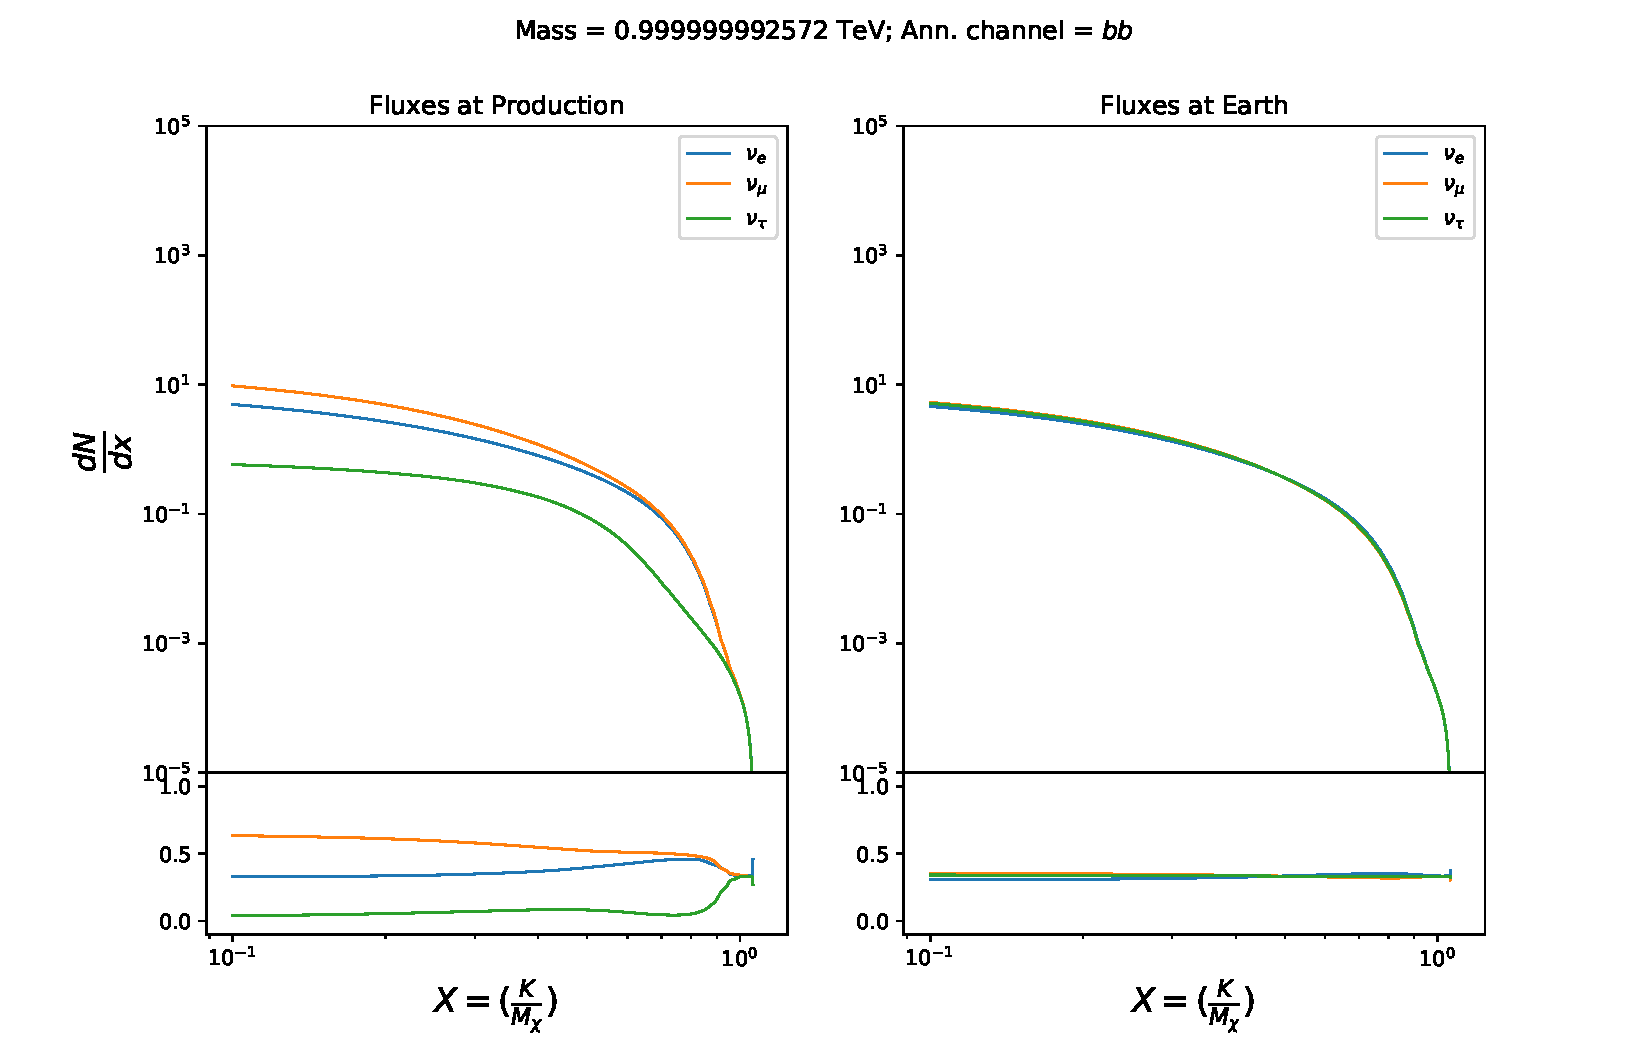
\includegraphics[scale=0.275]{figures/ic_DM/nu_spectra_bb_1.0000TeV.pdf}} &
        \raisebox{-.5\height}{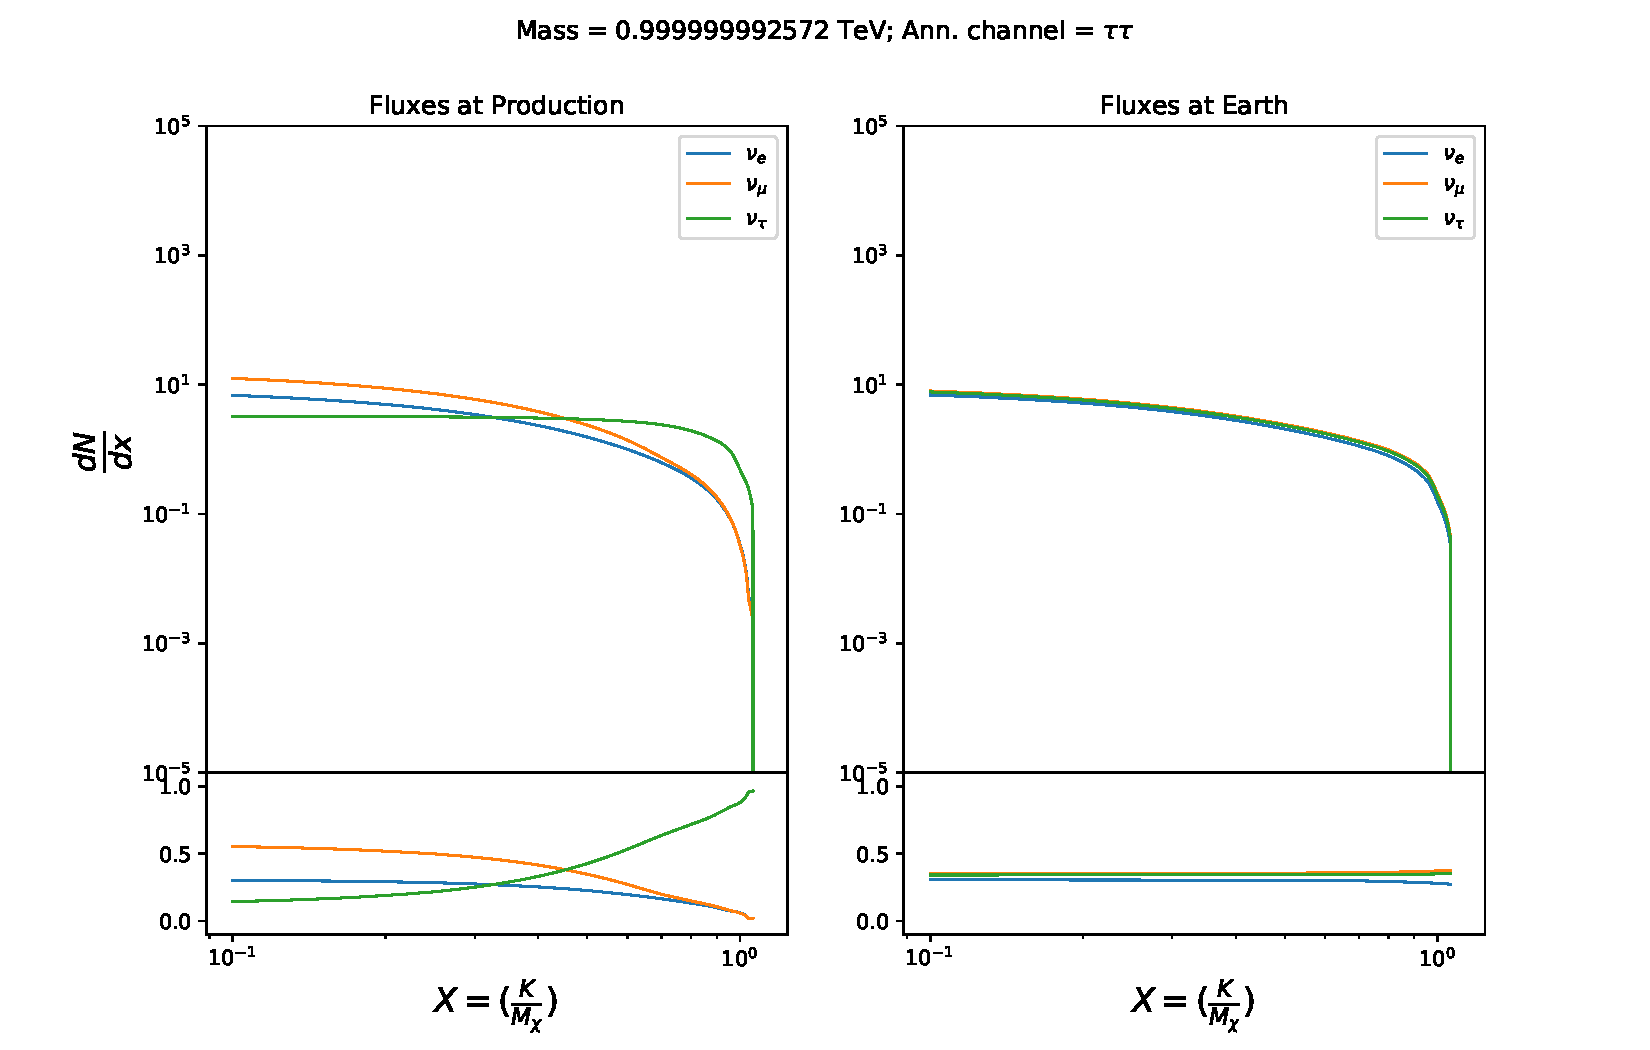
\includegraphics[scale=0.275]{figures/ic_DM/nu_spectra_tautau_1.0000TeV.pdf}} &
        \raisebox{-.5\height}{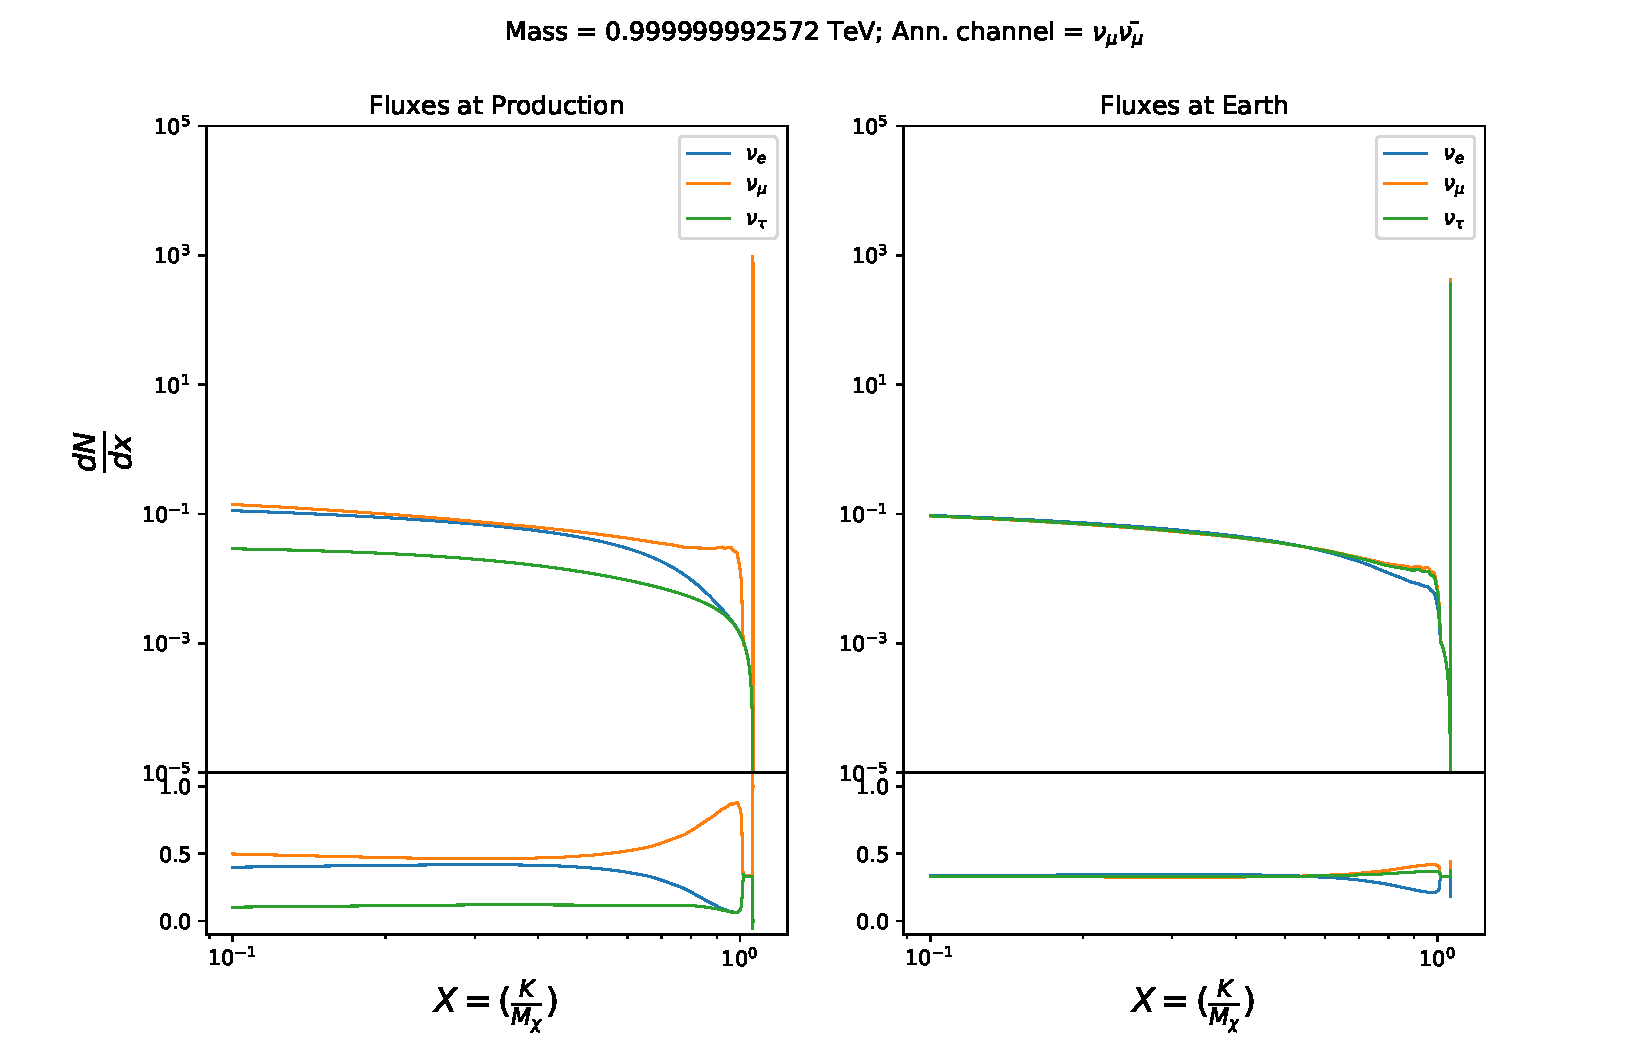
\includegraphics[scale=0.275]{figures/ic_DM/nu_spectra_numunumu_1.0000TeV.pdf}} \\

        \rotatebox[origin=c]{90}{1 PeV} &
        \raisebox{-.5\height}{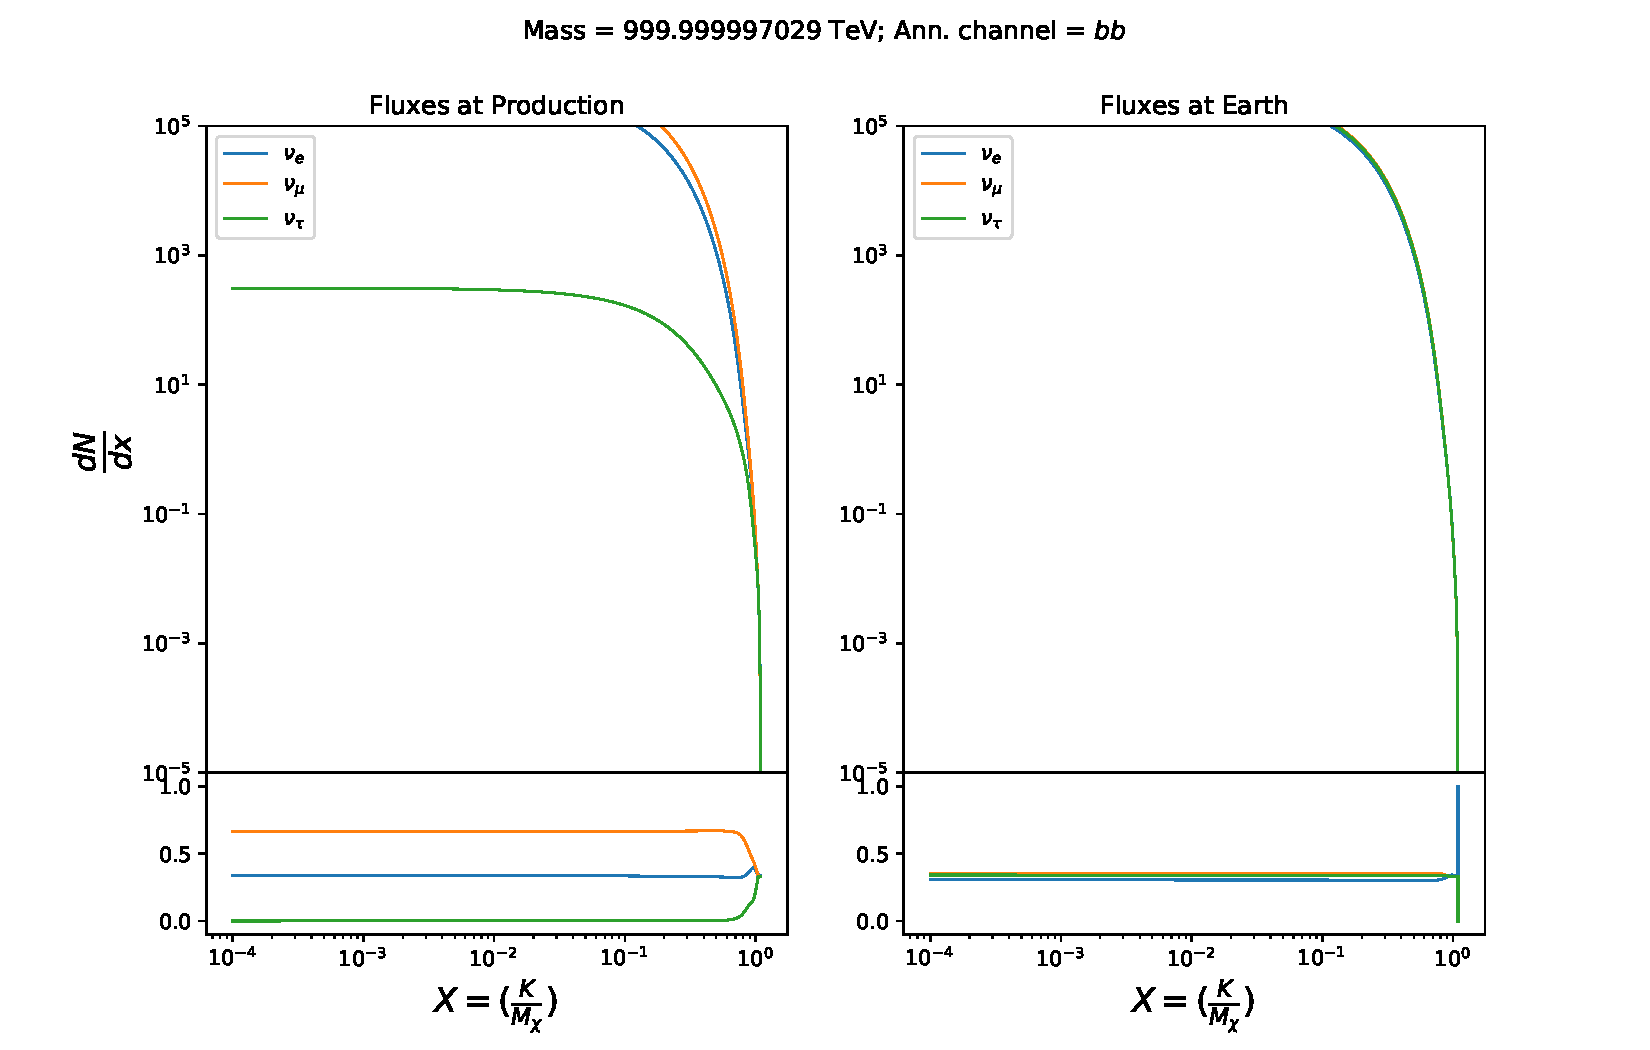
\includegraphics[scale=0.275]{figures/ic_DM/nu_spectra_bb_1000.0000TeV.pdf}} &
        \raisebox{-.5\height}{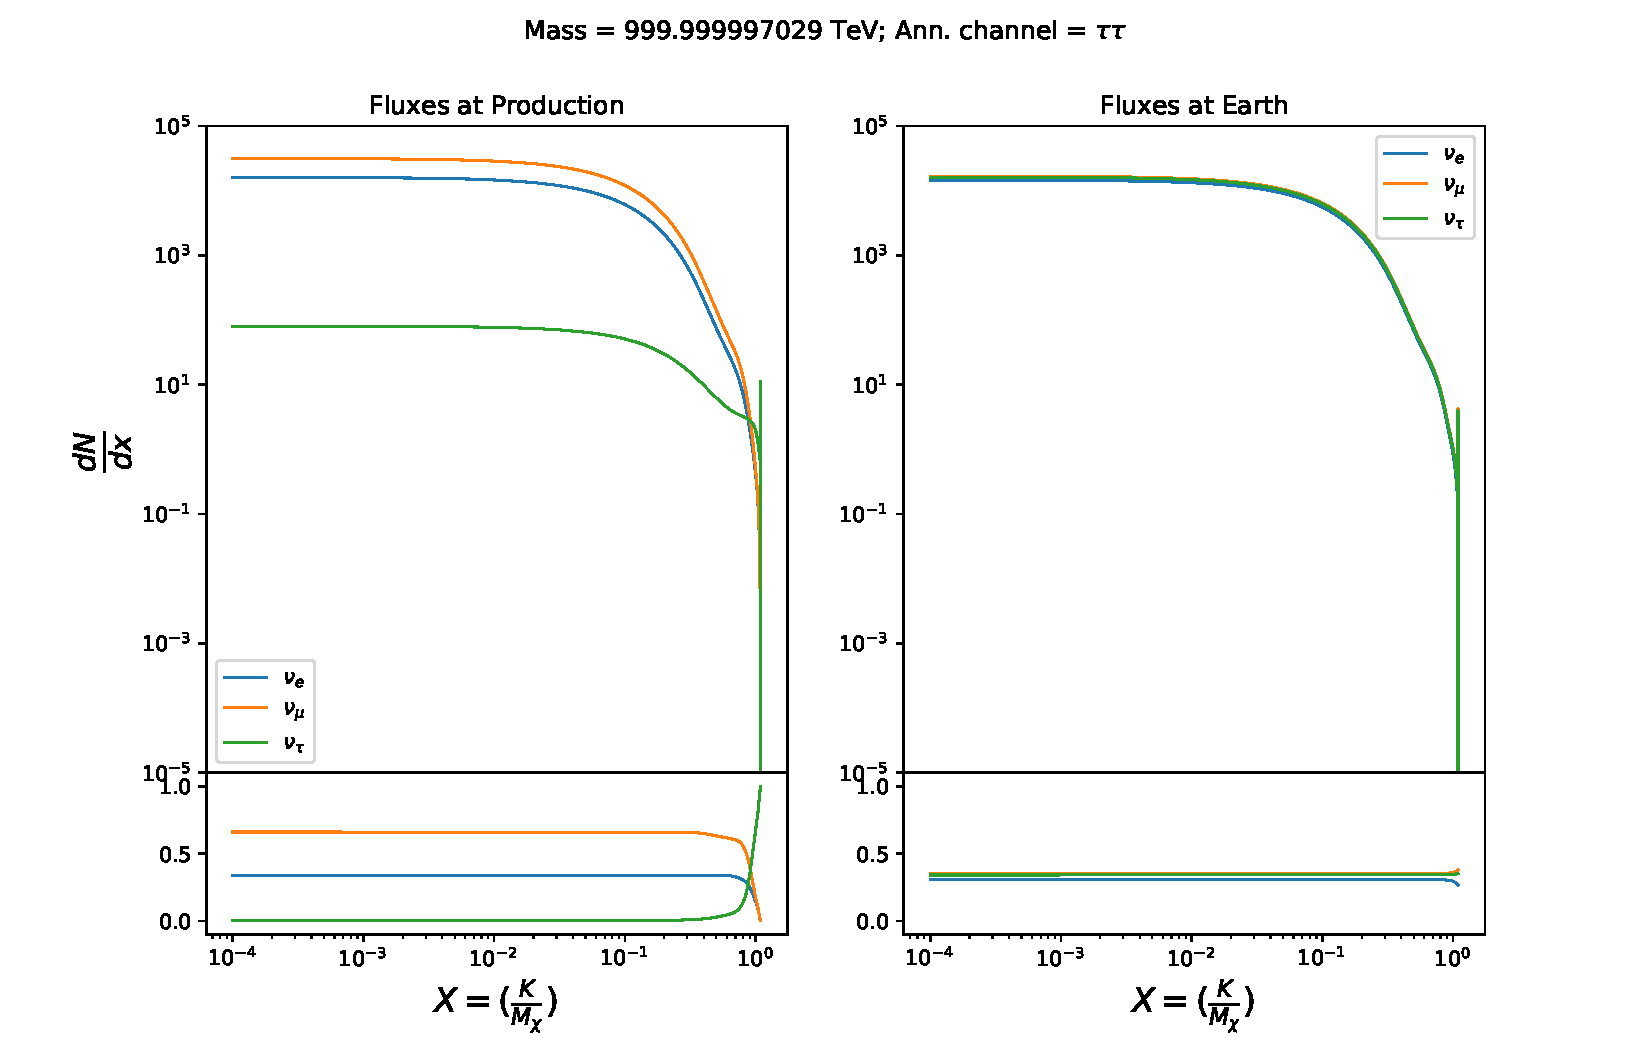
\includegraphics[scale=0.275]{figures/ic_DM/nu_spectra_tautau_1000.0000TeV.pdf}} &
        \raisebox{-.5\height}{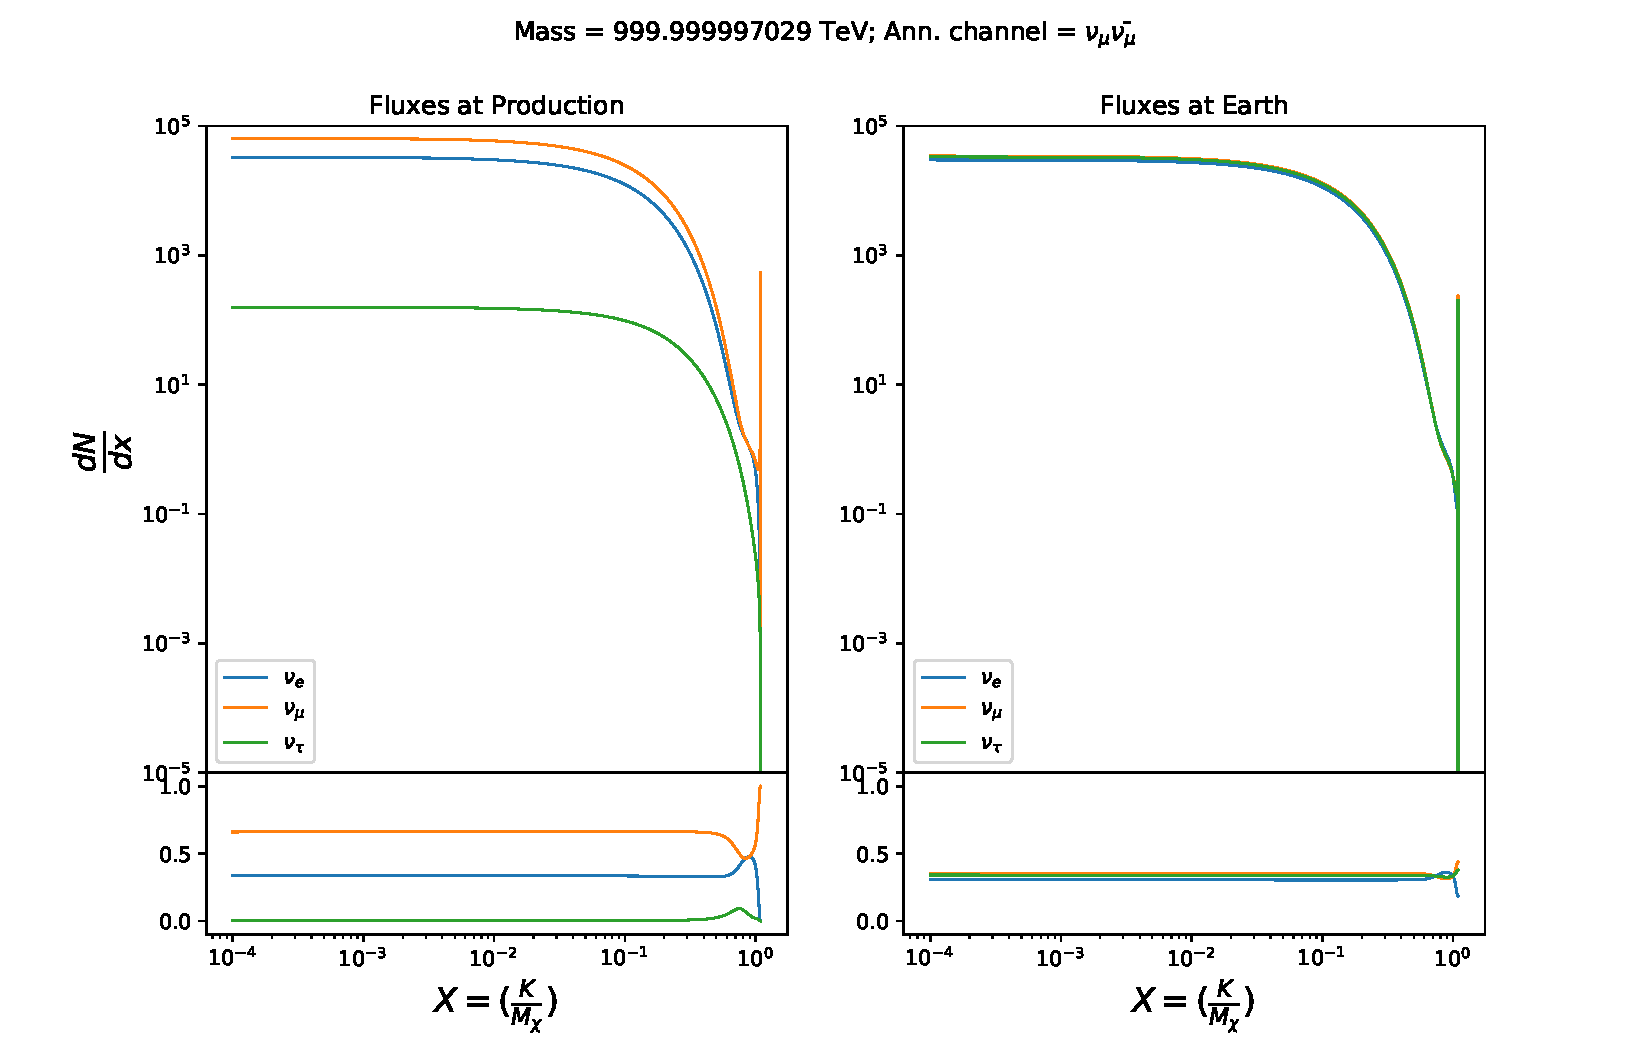
\includegraphics[scale=0.275]{figures/ic_DM/nu_spectra_numunumu_1000.0000TeV.pdf}} \\

        \rotatebox[origin=c]{90}{1 EeV} &
        \raisebox{-.5\height}{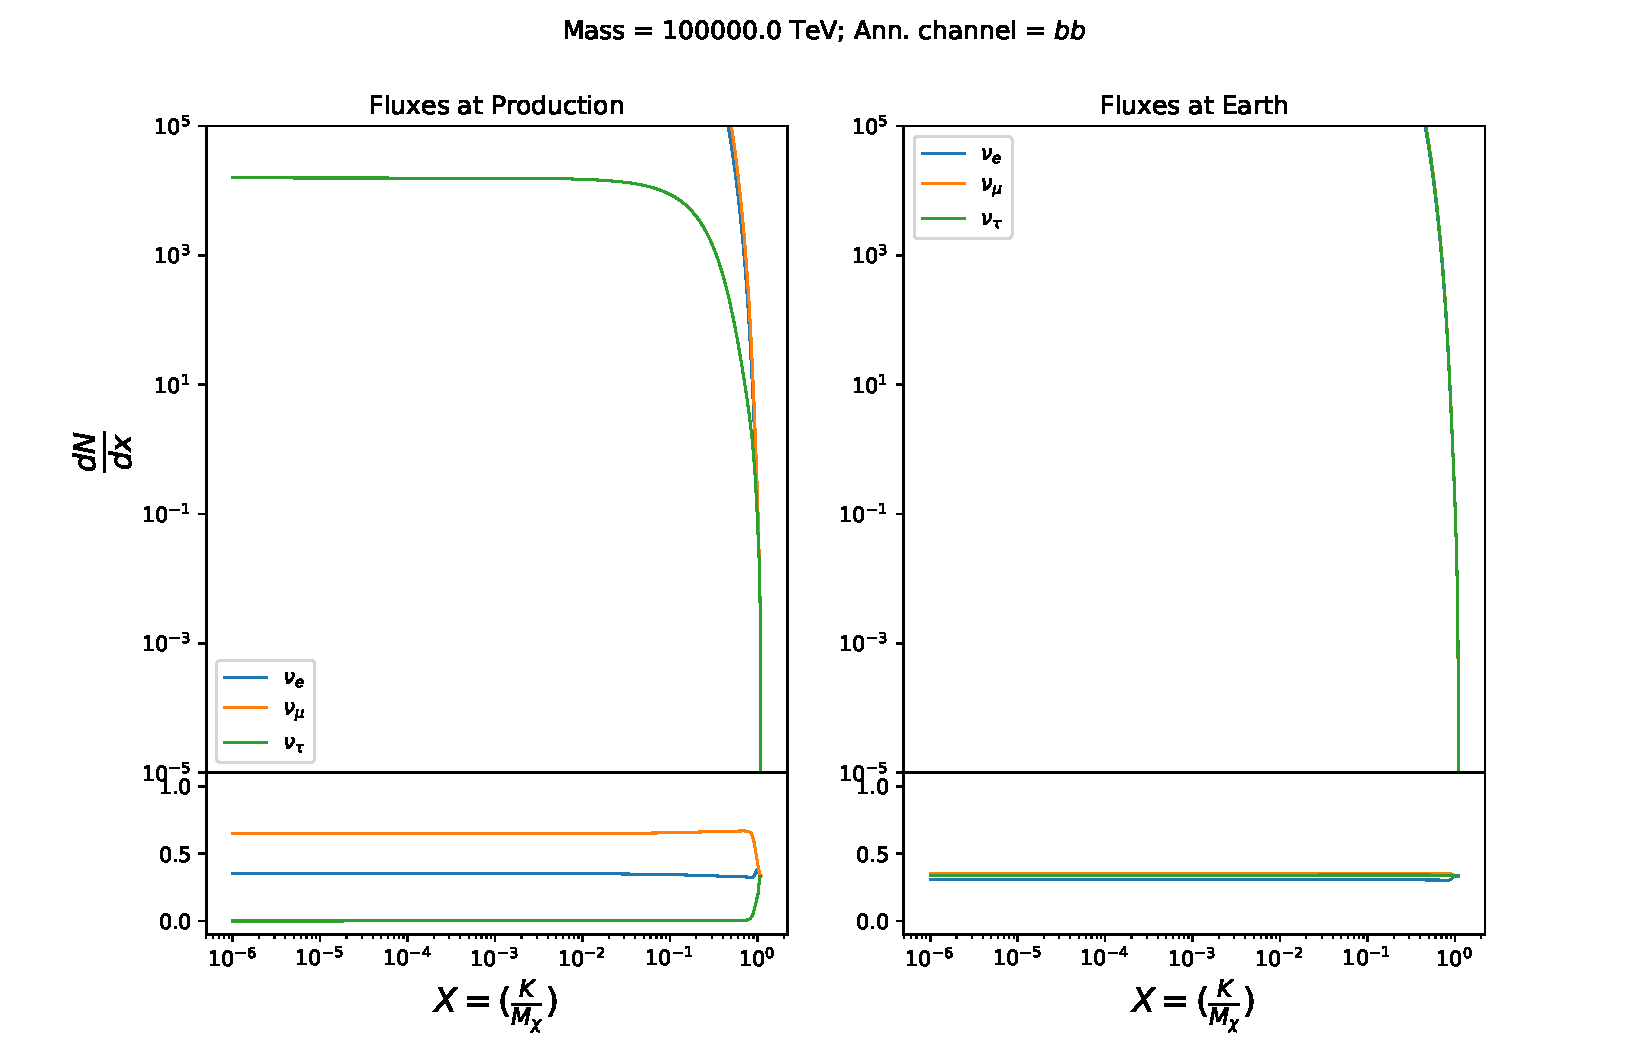
\includegraphics[scale=0.275]{figures/ic_DM/nu_spectra_bb_100000.0000TeV.pdf}} &
        \raisebox{-.5\height}{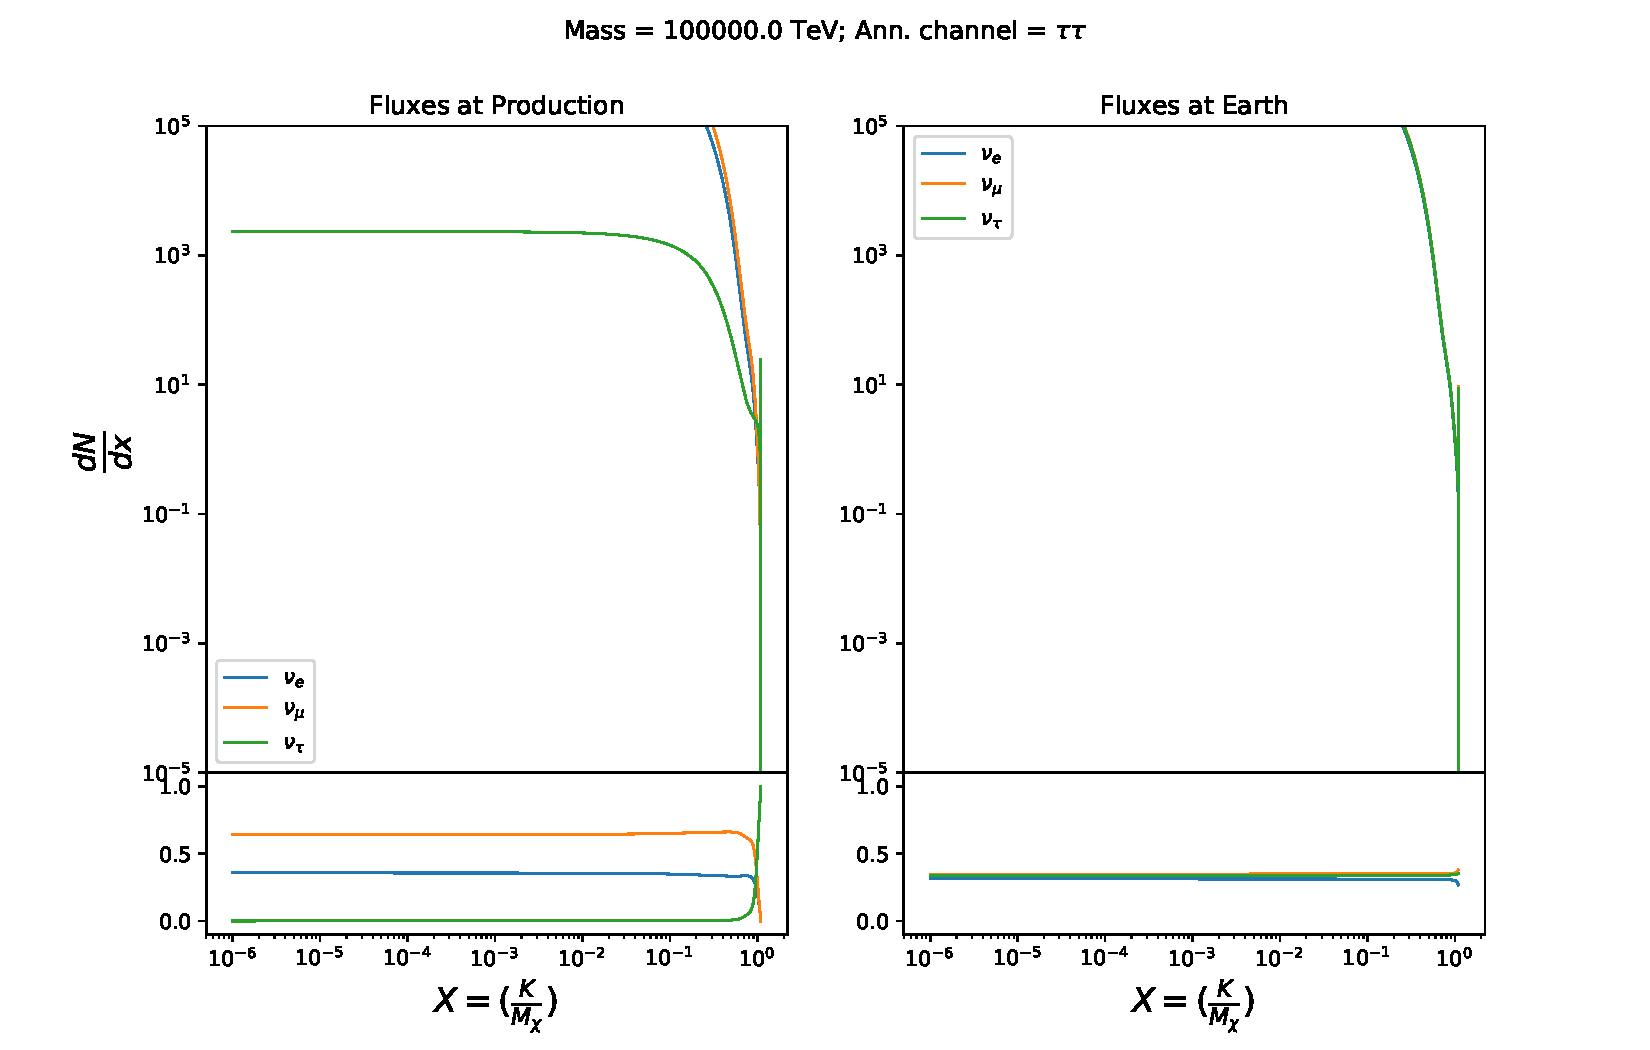
\includegraphics[scale=0.275]{figures/ic_DM/nu_spectra_tautau_100000.0000TeV.pdf}} &
        \raisebox{-.5\height}{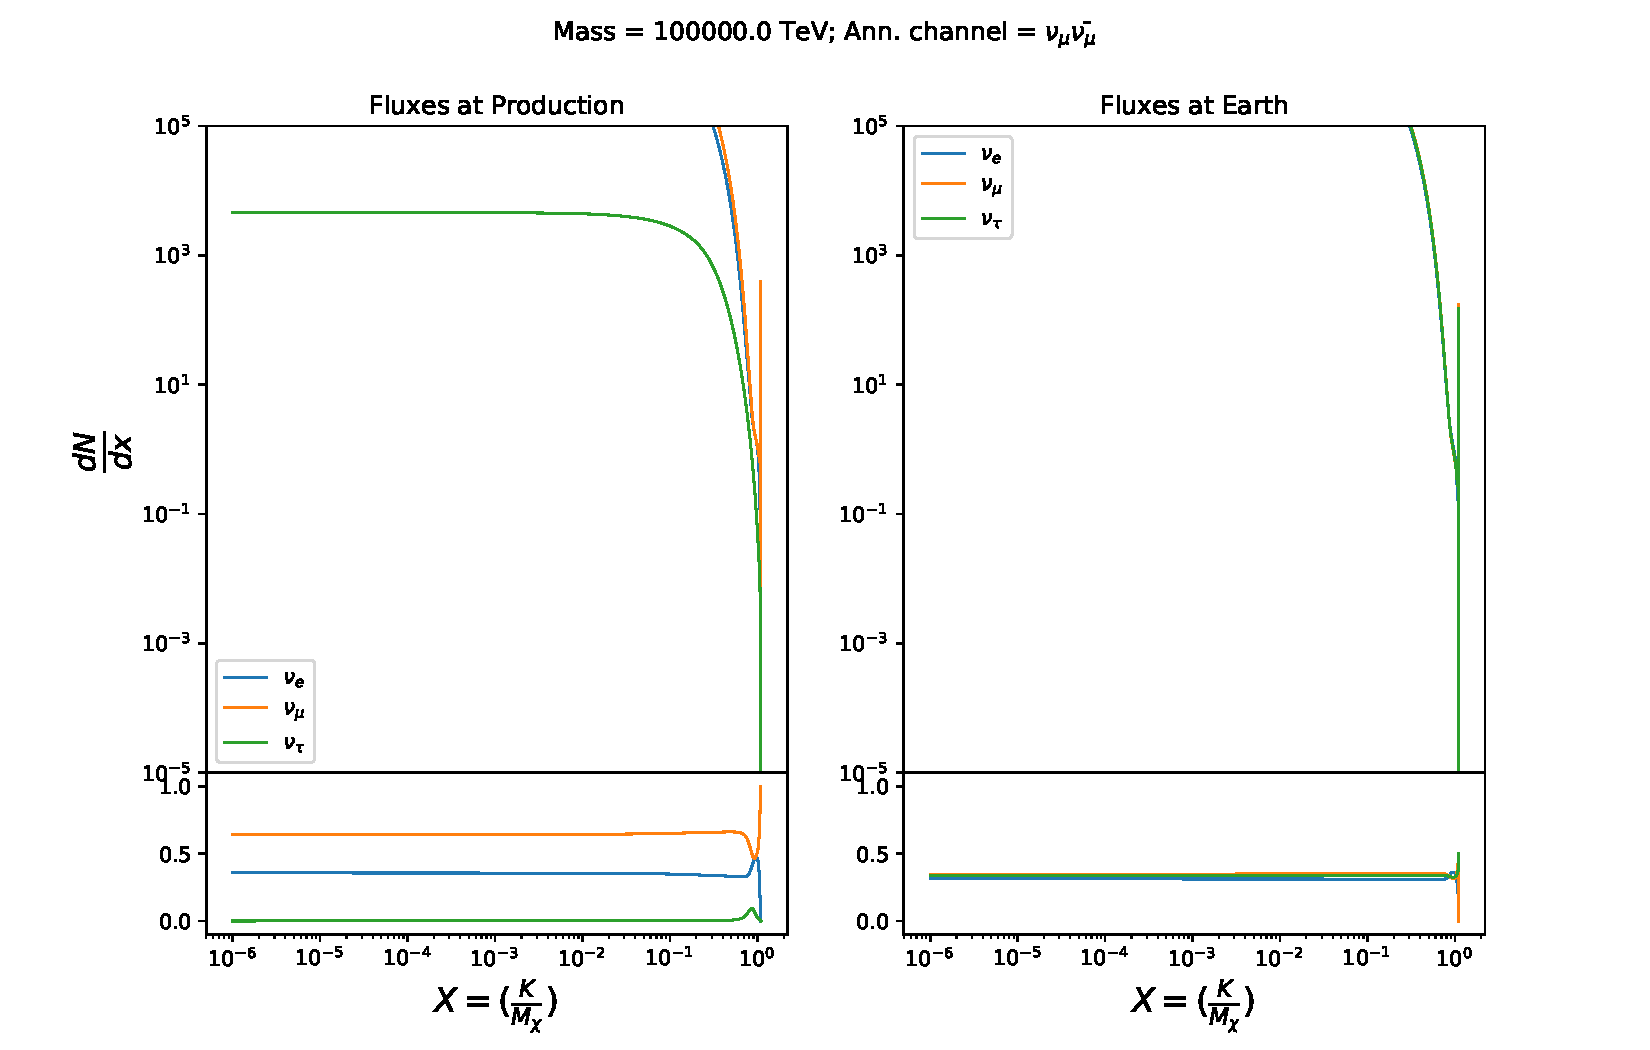
\includegraphics[scale=0.275]{figures/ic_DM/nu_spectra_numunumu_100000.0000TeV.pdf}} \\
    \end{tabular}
    \caption{Neutrino spectra at production (left panels) and after oscillation at Earth (right panels). Blue, orange, and green lines are the $\nu_e$, $\nu_\mu$, and $\nu_\tau$ spectra respectively. Top panels show the spectra in $\frac{dN}{dE}$. Lower panels plot the flavor ratio to $\nu_e + \nu_\mu + \nu_\tau$. SM annihilation channels \parpar{b}, \parpar{\tau}, and \parpar{\nu_\mu} are shown for $M_\chi =$ 1 Pev, TeV, and EeV.}
    \end{table}\label{fig:nu_osc_dm}
}
\end{landscape}
}

%%%%%%%%%%%%%%%%%%%%%%%%%%%%%%%%%%%%%%%%%%%%%%%%%%
\subsubsection{Treatment of Neutrino Line Features}\label{sec:icDM_nu_lines}
%%%%%%%%%%%%%%%%%%%%%%%%%%%%%%%%%%%%%%%%%%%%%%%%%%

All leptonic DM annihilation channels $ \chi\chi \rightarrow [\nu_{e, \mu, \tau}, e, \mu,\tau] $ develop a prominent and narrow spectral line feature.
For all neutrino flavors, this line is visible and prominent in all mass models studied for this analysis.
For charged leptons, the feature only really shows up at the larger DM mass models.
Examples for lines in both neutrinos and charged leptons annihilation are provided in \cref{fig:icDM_osc_dm}.
This line feature is so narrow relative the sampled energy range that the MC rarely samples within the neutrino line.
As a result, often the best fit to simulation of background will always floor to TS = 0 and the signal recovery tends to be conservatve.

\begin{figure}[t]
    \centering{
        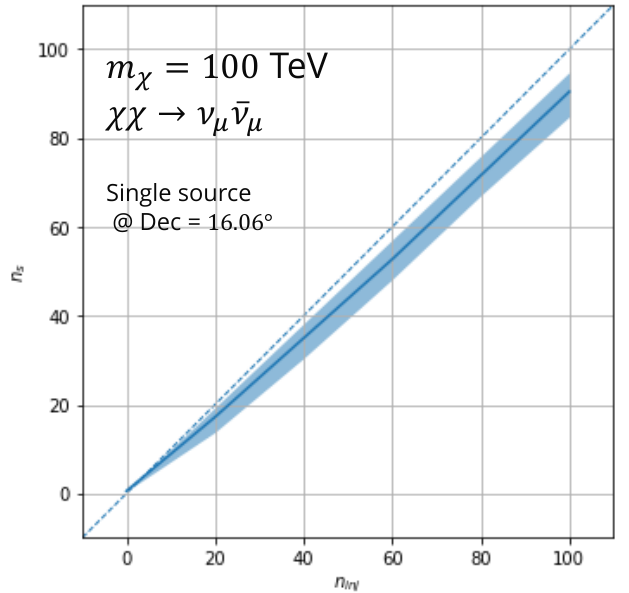
\includegraphics[scale=0.5]{figures/ic_DM/Sig_recover_line.png}
    }
    \caption{Signal recovery for 100 TeV DM annihilation into \parpar{\nu_\mu} for a source at Dec = 16.06$^\circ$. $n_\mathrm{inj}$ is the number of injected signal events in simulation. $n_s$ is the number of reconstructed signal events from the simulation. Although the uncertainties are small and tight, the reconstructed $ n_s $ are systematically underestimated.} \label{fig:sig_recovery_fail}
\end{figure}


To remedy this, a similar approach to the IceCube's decay analysis \todo{refer to Minjin's page}.
2 kernels were tested (Gaussian, uniform (flat)) to smooth out the line feature.
The widths were tuned such that the signal recovery approached unity for DM mass 100 TeV to 1 PeV.
Additionally, the tuning was performed only for a source at declination 16.06 (Segue 1).
This is to avoid confusion loss in signal recovery from too narrow a line and from Earth's attenuation of high energy neutrinos.
The convolution also needed to as close as possible preserve the integrated counts of neutrinos.
The optimized kernel window for all lines is summarized as:
\begin{itemize}
    \item Guassian kernel w/$2 \sigma$ width = 3.5E-3$\cdot m_\chi$
    \item Minimum energy included in convolution = MIN$[0.995 \cdot m_\chi, En(\nu_{line}) -4\sigma]$
    \item Maximum energy included in convolution = MAX$[1.005 \cdot m_\chi, En(\nu_{line}) +4\sigma]$
\end{itemize}
where $En(\nu_{line})$ is the neutrino energy where the neutrino line is at the maximum.

\begin{figure}[h]
    \centering{

    \begin{tabular}{cc}
        \begin{tabular}{cc}
            \rotatebox[origin=c]{90}{\small{\todo{Check y axe}}} &
            \raisebox{-.5\height}{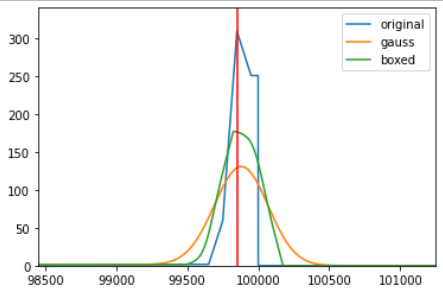
\includegraphics[scale=0.5]{figures/ic_DM/sig_recovery_fixed copy.png}} \\

            &
            \small{$E_\nu$ (GeV)} \\
        \end{tabular} &

        \raisebox{-.5\height}{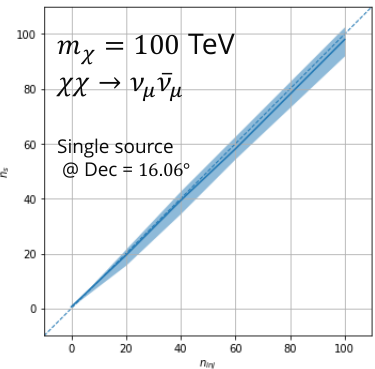
\includegraphics[scale=0.5]{figures/ic_DM/sig_recovery_fixed.png}} \\
    \end{tabular}
    }\caption{Top left panel shows the two kernels overlayed the original spectrum from Charon. delta I is the difference in the integral of the peaks with respect to the original spectrum. The vertical red line indicated where the original neutrino line is maximized. Lower right shows the signal recovers of the DM model using the Gaussian kernel with parameters enumerated above.} \label{fig:icDM_fixed_line}
\end{figure}

These parameters broadly improved the signal recovery of the line spectra.
An example is provided below.
Signal recovery plots of the full analysis are provided much further down.

%%%%%%%%%%%%%%%%%%%%%%%%%%%%%%%%%%%%%%%%%%%%%%%%%%
\subsubsection{Spline Fitting}\label{sec:icDM_splines}
%%%%%%%%%%%%%%%%%%%%%%%%%%%%%%%%%%%%%%%%%%%%%%%%%%

In an effort to reduce computational work, memory burden, and align with point source methods used for NGC1068 and Seyfert analyses, spectral splines were created and adopted for estimating the neutrino flux for the different annihilation.
Software was written to generate, handle, and calculate values on the splines.
When using splines, one has to be careful of the goodness to fit.
There are critical caveats when testing the goodness to fit to MC generated above for all channels.
\begin{itemize}
    \item The splines must be Log10(*) in Energy and dN/dE to acount for the exponential nature of the flux
    \item The fidelity of the fit matters more at $ E_\nu \thickapprox m_\chi $ where the model uncertainties are minimal and physical considerations (like the cut-off) are most apparent.
    \item The fidelity of the fit matters less at low $ E_\nu $ as the model uncertainties are large AND IceCube's sensitivity diminishes significantly below 500 GeV
    \item Total integrated counts should be well preserved, however, the resolution of the MC is much higher than IceCube's energy resolution.
    \begin{itemize}
        \item Meaning over several steps in E, the integral is preserved
        \item the step size enters the cost function
        \item Oscillating residuals, so long as they are very small and well centered, are not penalized as this gets averaged out.
    \end{itemize}
\end{itemize}

The resulting cost function to evaluate the goodness of fit was used to account for the above considerations.
\erriSpline

Where $ \hat{e_i} $ is the spline estimator's value for $x_i$. $ x_i = E_{\nu_i} / m_\chi $. $ \frac{dN_i}{dE_i} $ is the flux value from MC.
\MSEspline

I then take the RMS of the error distribution and the resulting value (err) is used to evaluate the fidelity of the spectral spline.
Each SM channel had different tolerances for 'err'. Channels with very hard cut-offs had looser tolerance for err because a lot of error would be generated from the cut-off being estimated to occur slightly early or late.
Soft channels don't have this issue and therefore the tolerance is very strict.
The table blow summarizes the tolerances for the SM channels.
\begin{table}
    \centering{
    \begin{tabular}{c|c c c c}
        \hline
        $ \chi\chi \rightarrow $ &
        GOOD &
        OK   &
        FAIL &
        Limits of err calc [$X_{min}, X_{max}$] \\
        \hline
        \hline

        $ Z^0Z^0, W^+W^- $ &
        $1.0 \cdot 10^{-3}$ &
        \makecell{$1.0 \cdot 10^{-3}$, \\ $1.0 \cdot 10^{-2}$} &
        $1.0 \cdot 10^{-2}$ &
        MAX$[100 \mathrm{GeV}/m_\chi, 10^{-6}], 1.0 $ \\
        \hdashline

        $ t\bar{t}, hh $ &
        $1.0 \cdot 10^{-5}$ &
        \makecell{$1.0 \cdot 10^{-5}$, \\ $1.0 \cdot 10^{-4}$} &
        $1.0 \cdot 10^{-4}$ &
        MAX$[100 \mathrm{GeV}/m_\chi, 10^{-6}], 1.0 $ \\
        \hdashline

        $ b\bar{b}, d\bar{d}, u\bar{u}$ &
        $9.0 \cdot 10^{-7}$ &
        \makecell{ $9.0\cdot 10^{-7}$, \\ $9.0 \cdot 10^{-6}$} &
        $9.0 \cdot 10^{-6}$ &
        MAX$[100 \mathrm{GeV}/m_\chi, 10^{-6}], 1.0 $ \\
        \hdashline

        $ \nu\bar{\nu}_{e, \mu, \tau} $ &
        $1.0 \cdot 10^{-3}$ &
        \makecell{$1.0 \cdot 10^{-3}$, \\ $1.0 \cdot 10^{-2}$} &
        $1.0 \cdot 10^{-2}$ &
        \makecell{MAX$[100 \mathrm{GeV}/m_\chi, 10^{-6}]$, \\ MIN$[0.995, (E_{\nu_{line}}) -4\sigma)/M_{\chi}] $} \\
        \hdashline

        $ e\bar{e}, \mu\bar{\mu}, \tau\bar{\tau} $ &
        $1.0 \cdot 10^{-3}$ &
        \makecell{$1.0 \cdot 10^{-3}$, \\ $1.0 \cdot 10^{-2}$}&
        $1.0 \cdot 10^{-2}$ &
        \makecell{MAX$[100 \mathrm{GeV}/m_\chi, 10^{-6}]$, \\ MIN$[0.995, (E_{\nu_{line}}) -4\sigma)/M_{\chi}]$} \\

    \end{tabular}
    }
    \caption{Spline err tolerances used for input in particle physics component to \cref{eq:id_dm_flux}. Column 1 is the DM annihilation channel being fit. Columns 2, 3, and 4 are the tolerances for "GOOD" (pass), "OK" requires inspection, and "FAIL" (tune and refit) respectively. Column 5 has the X ranges over which the error is evaluated. MAX/MIN [$\cdot$,$\cdot$] takes the maximum or minumum of the two enclosed values.} \label{tab:spline_tolerance}
\end{table}

The errors are then plotted in two ways.
First, FAIL and OK are directly plotted with $e_i$ as a function of x, and the full spline and MC.
Second, a summary plot of all the splines is plotted and colors coded.

\begin{figure}
    \centering{
    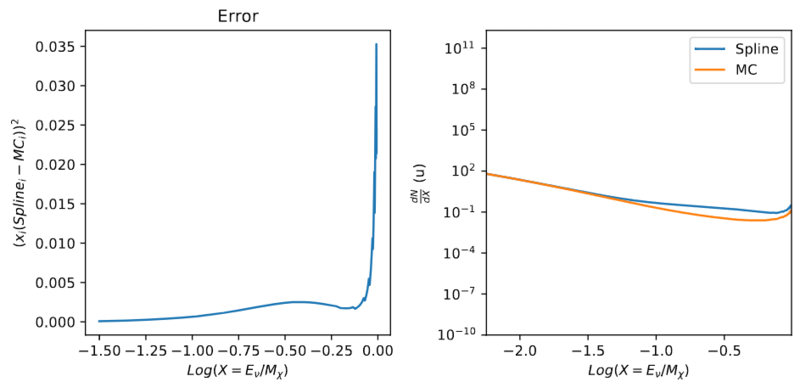
\includegraphics[scale=0.6]{figures/ic_DM/800px-Failed_spline.png}
    }
    \caption{Example spline that failed the fit. Failed splined are corrected on a case by case basis unless the SM channel has a systematic problem fitting the splines. In this case, I made a bookkeeping error and loaded the incorrected neutrino flavor}
    \label{fig:icDM_failedspline}
\end{figure}

\Cref{fig:apdx_nu_splines} are the spline summaries and represent the current, up-to-date status of the splines.
The goal broadly is to eliminate all red and inspect yellow. $ \nu_e $ is not considered in this analysis among the neutrino final states and so no work was done to converge the spline fits for this flavor.

A Final inspection of the splines by eye was done to verify that the spline fitting did not introduce spurious features into the distribution that would corrupt the LLH fitting.

%%%%%%%%%%%%%%%%%%%%%%%%%%%%%%%%%%%%%%%%%%%%%%%%
\subsubsection{Composite Neutrino Spectra}\label{sec:icDM_composite_dNdE}
%%%%%%%%%%%%%%%%%%%%%%%%%%%%%%%%%%%%%%%%%%%%%%%

With all of the previously mentioned pieces, we are ready to fully assemble a comprehensive description of the particle physics term $dN/dE$ in \cref{eq:id_dm_flux}.
\nuIDDMFlux

Presented below are the final spectra that are used in the DM analysis. Bluer spectra are for lower DM mass models. The redder, the higher the DM mass.
Energy (x-axis) was chosen to roughly represent the energy sensitivity of NST.
These spectra are the composite (nu and tau flavors) versions. How these are combined is mentioned earlier.

\tmpfig{Show the post processed spectra that you are sampling}

%
% <center>
% {|class="wikitable" style="border-spacing: 2px; border: 1px solid darkgray;"
% |+ Output composite spectra after spline fit and line smoothing
% |-
% | <center> $ \chi\chi \rightarrow b\bar{b} $ </center>
% | <center> $ \chi\chi \rightarrow t\bar{t} $ </center>
% | <center> $ \chi\chi \rightarrow \nu_{\mu}\overline{\nu_{\mu}} $ </center>
% |-
% | [[Image:bb_rainbow.png |300px]]
% | [[Image:tt_rainbow.png |300px]]
% | [[Image:numu_rainbow.png |300px]]
% |-
% | <center> $ \chi\chi \rightarrow W^+ W^- $ </center>
% | <center> $ \chi\chi \rightarrow Z^0Z^0 $ </center>
% | <center> $ \chi\chi \rightarrow \nu_{\tau}\overline{\nu_{\tau}} $ </center>
% |-
% | [[Image:ww_rainbow.png |300px]]
% | [[Image:zz_rainbow.png |300px]]
% | [[Image:nutau_rainbow.png |300px]]
% |-
% | <center> $ \chi\chi \rightarrow \nu_{e}\overline{\nu_{e}} $ </center>
% |-
% | [[Image:nue_rainbow.png |300px]]
% |}
% </center>
%
%%%%%%%%%%%%%%%%%%%%%%%%%%%%%%%%%%%%%%%%%%%%%%%%%%
\subsection{\J - Astrophysical Component}\label{sec:icDM_spatialmodel}
%%%%%%%%%%%%%%%%%%%%%%%%%%%%%%%%%%%%%%%%%%%%%%%%%%

The expected neutrino counts from a dwarf spheroidal galaxy depends also on the the 'astrophysical factor'.
The value for this (in our specific case) J-factor for a target depends on its dark matter density distribution, $\rho_{\chi}$ and how far it is $ l $.
For this analysis, we adopt the \GS model used in \cref{sec:glory_duck} for dSph from \cite{Geringer_Sameth_2015}.
These models are based on a modified Navarro-Frenk-While (NFW) profile where the indices of the NFW (traditionally 1,3,1) are allowed to float.
More specifically, these DM distributions are described using the Zhao profile.
The Zhao profile is written as:

%
% <center>
% $
% \rho_{Zhao}(r; r_{s}, \rho_{s}, \alpha, \beta, \gamma) = \frac{\rho_{s}}{\left(\frac{r}{r_{s}}\right)^{\gamma} \left[1 + \left(\frac{r}{r_{s}}\right)^{\alpha} \right]^{(\beta-\gamma)/\alpha}  }
% $,
% </center>
% where $ r_{s} $, $\rho_{s}$ denote scale radius, scale density respectively. According to these models, the dark matter distributions of the sources are spherically symmetric. Hence, the J-factor is calculated as the following :
% <center>
% $
%
% J(\theta) = 2 \pi \int_{0}^{\theta} \sin \theta^{'} d\theta^{'} \int^{\infty}_{0}dl^{'} \rho^2_{\chi}(r[l^{'}, \theta^{'}])
%
% $,
% </center>

where $ \theta $ is the angular distance from the center of the source.
For the case annihilation, the source diameter, [https://iopscience.iop.org/article/10.1088/0004-637X/801/2/74 here] defined as the $ 2 \theta_{\mathrm{max}} $ , of these dwarves is typically under $ 1^{\circ} $ with the largest in the catalog, Fornax, extending to $ 2.61^{\circ} $.
Fornax is not in the northern sky and the remaining sources are notably below this angular size.
Therefore, the sources are treated as point sources because the typical source diameter is under 1 degree.
The J-factor used for the point source assumption is the total J emitted from $ \theta_{\mathrm{max}} $.
These values are enumerated in Geringer-Sameth 2015 and again in the table below with their coordinates.
Coordinates are given in J200.0 equatorial coordinates.
IceCube uses identical sources to \cref{tab:gd_J_factor} except we analyze source with declinations above 0.0 degrees.

%%%%%%%%%%%%%%%%%%%%%%%%%%%%%%%%%%%%%%%%%%%%%%%%%%
\subsection{Source Selection and Annihilation Channels}\label{sec:ic3_study_selection}
%%%%%%%%%%%%%%%%%%%%%%%%%%%%%%%%%%%%%%%%%%%%%%%%%%

We use all of the dSphs presented in IceCube's previous dSph DM search \cite{IC3_DM2013}.
IceCube's sources for these simulation studies include Bootes I, Canes VenaticiI, Canes Venatici II, Coma Berenices, Draco, Hercules, Leo I, Leo II, Leo V, Leo T, Segue 1, Segue 2, Ursa Major I, Ursa Major II,  and Ursa Minor.
A full description of all sources used in \Cref{tab:gd_J_factor}.
Sources with declinations less than 0.0 are excluded from this analysis.

This analysis improves on the previous IceCube dSph paper \cite{IC3_DM2013} in the following ways.
Previously, the IceCube detector was not yet completed to the 86 string configuration.
Many more dSphs will be observed, from 4 to 15.
Previously, the particle physics model used for neutrino-ray spectra from DM annihilation did not have EW corrections where they are now included \cite{HDMSpectra}.
The spectral models also predict substantial differences between the neutrino flavors, so this analysis will be the first DM dwarf analysis to discriminate betwen primary neutrino flavors.
The study performed here studies 10.4 years of data.

The SM annihilation channels probed for this study include \parpar{b}, \parpar{t}, \parpar{u}, \parpar{d}, \parpar{e}, \parpar{\mu}, \parpar{\tau}, \pp{Z}, $W^+W^-$, \parpar{\nu_e}, \parpar{\nu_\mu}, and \parpar{\nu_\tau}.

%%%%%%%%%%%%%%%%%%%%%%%%%%%%%%%%%%%%%%%%%%%%%%%%%%
\section{Likelihood Methods}\label{sec:icDM_LLH}
%%%%%%%%%%%%%%%%%%%%%%%%%%%%%%%%%%%%%%%%%%%%%%%%%%

I use the Point-Source search likelihood which is widely used in IceCube analyses.
The likelihood function is defined as the following:
\icPtSrcLLH
where  $ i $ is an event index, $S$ and $B$ are the signal PDF and background PDF respectively. For a joint analysis where the sources are stacked the likelihood is expanded in the simplified way:
\icStackLLH
Where $ L_i $ is the likelihood from the i-th source in the stacked analysis.
The test statistic definition remains the same as \cref{eq:gd_TS}


%%%%%%%%%%%%%%%%%%%%%%%%%%%%%%%%%%%%%%%%%%%%%%%%%%
\section{Background Simulation}\label{sec:icDM_bkgd_sim}
%%%%%%%%%%%%%%%%%%%%%%%%%%%%%%%%%%%%%%%%%%%%%%%%%%

Before we look at data, we must first analyze background and signal injection to validate our anlysis.
The following sections show the reults of the likelihood fitting for a suite of background trials for the DM models we set out to study in \todo{refer to the section}.
We study the TS distributions first for each source, then for the stacked analysis.

The TS distributions are not expected to behalf according to a chi-squared distribution with 1 degree of freedom.
This is in large part due to the distinct spectral shapes demonstrated earlier.
These can vary significantly between DM mass and annihilation models.
Therefor, Wilks' theorem may not be applicable to the analysis.
Instead, a critical value is defined from a large number of background trials.

I assume that TS values are physical: $ \mathrm{TS} \ge 0 $.
$\eta$ denotes the fraction of positive TS values above the threshold and written in the legend.
$ \epsilon[x] $ indicate the fraction of events where $ \mathrm{TS} < x $. For TS plots shown here, the decimal values of x are 1.0e-2 and 1.0e-3.
The following plots show the background TS distributions obtained from Segue1, a source with little Earth attenuation and large J-factor, assuming that dark matter annihilates into $b\overline{b}$.
I also show the 15 source stack TS distributions with identical DM models.

%%%%%%%%%%%%%%%%%%%%%%%%%%%%%%%%%%%%%%%%%%%%%%%%%%
\subsection{TS per Source} \label{sec:icDM_TSperSrc}
%%%%%%%%%%%%%%%%%%%%%%%%%%%%%%%%%%%%%%%%%%%%%%%%%%

Below I present the TS distributions for Segue1 and $ \chi\chi \rightarrow$ \parpar{b}. All remaining channels and source TS panels are hosted on \todo{Change this text, it will all be here}.

Although it was not expected, almost every distribution produced follows a chi2 distribution with 1 degree of freedom.
This is important for future assumptions made (in multi-messenger) and may justify statistical calculations assuming Wilk's theorem is valid.

\todo{add text saying that you show: bb, numu, and tau??? specs for Seg1 and UMa2? }

\begin{figure}[t]
    \centering{
        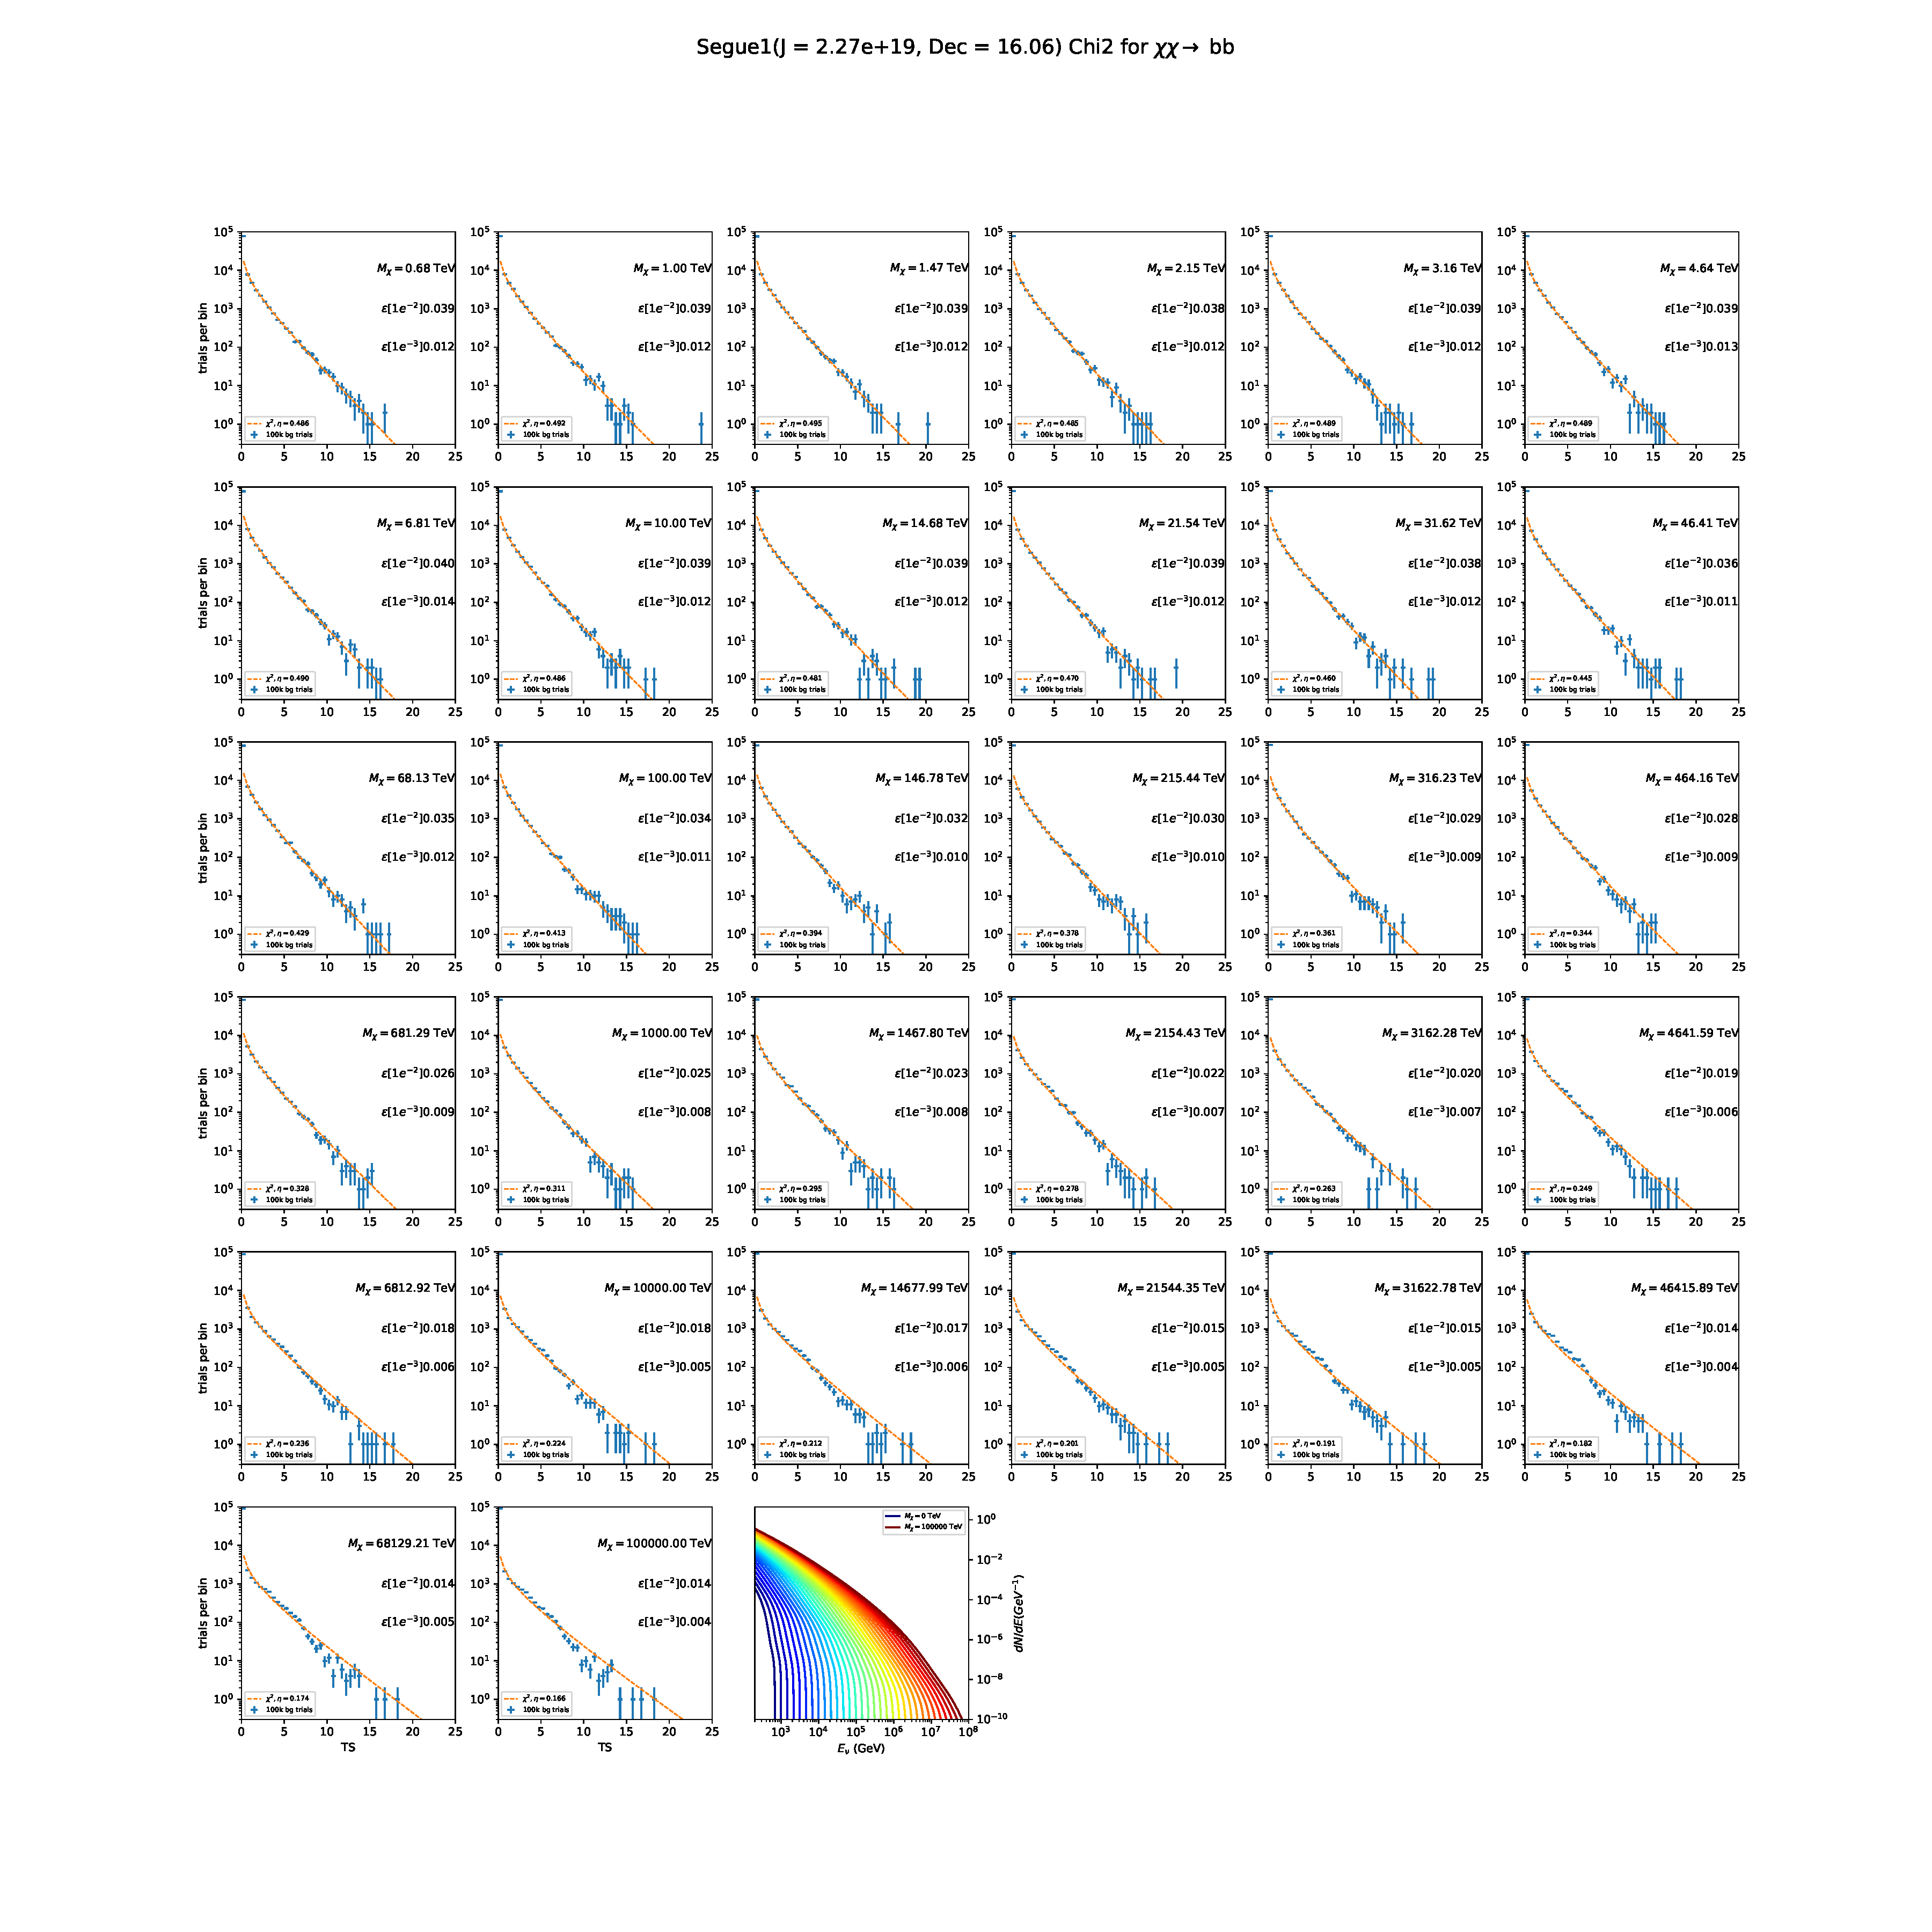
\includegraphics[clip, trim=5.7cm 5.2cm 5.7cm 6.7cm, scale=0.326]{figures/ic_DM/dm_plots/Segue1_bb_chi2_Masspanel.pdf}
    }\caption{\todo{update text because there is no title.} Each subplot, except the final, is the TS distribution for a specific DM mass listed in the subplot. The final subplot plots the all DM spectral models used as input for the TS distribution calculations with bluer lines indicating lower DM mass and redder indicating higher DM mass.}
    \label{fig:icDM_Seg1bb_TS}
\end{figure}

\begin{figure}[t]
    \centering{
        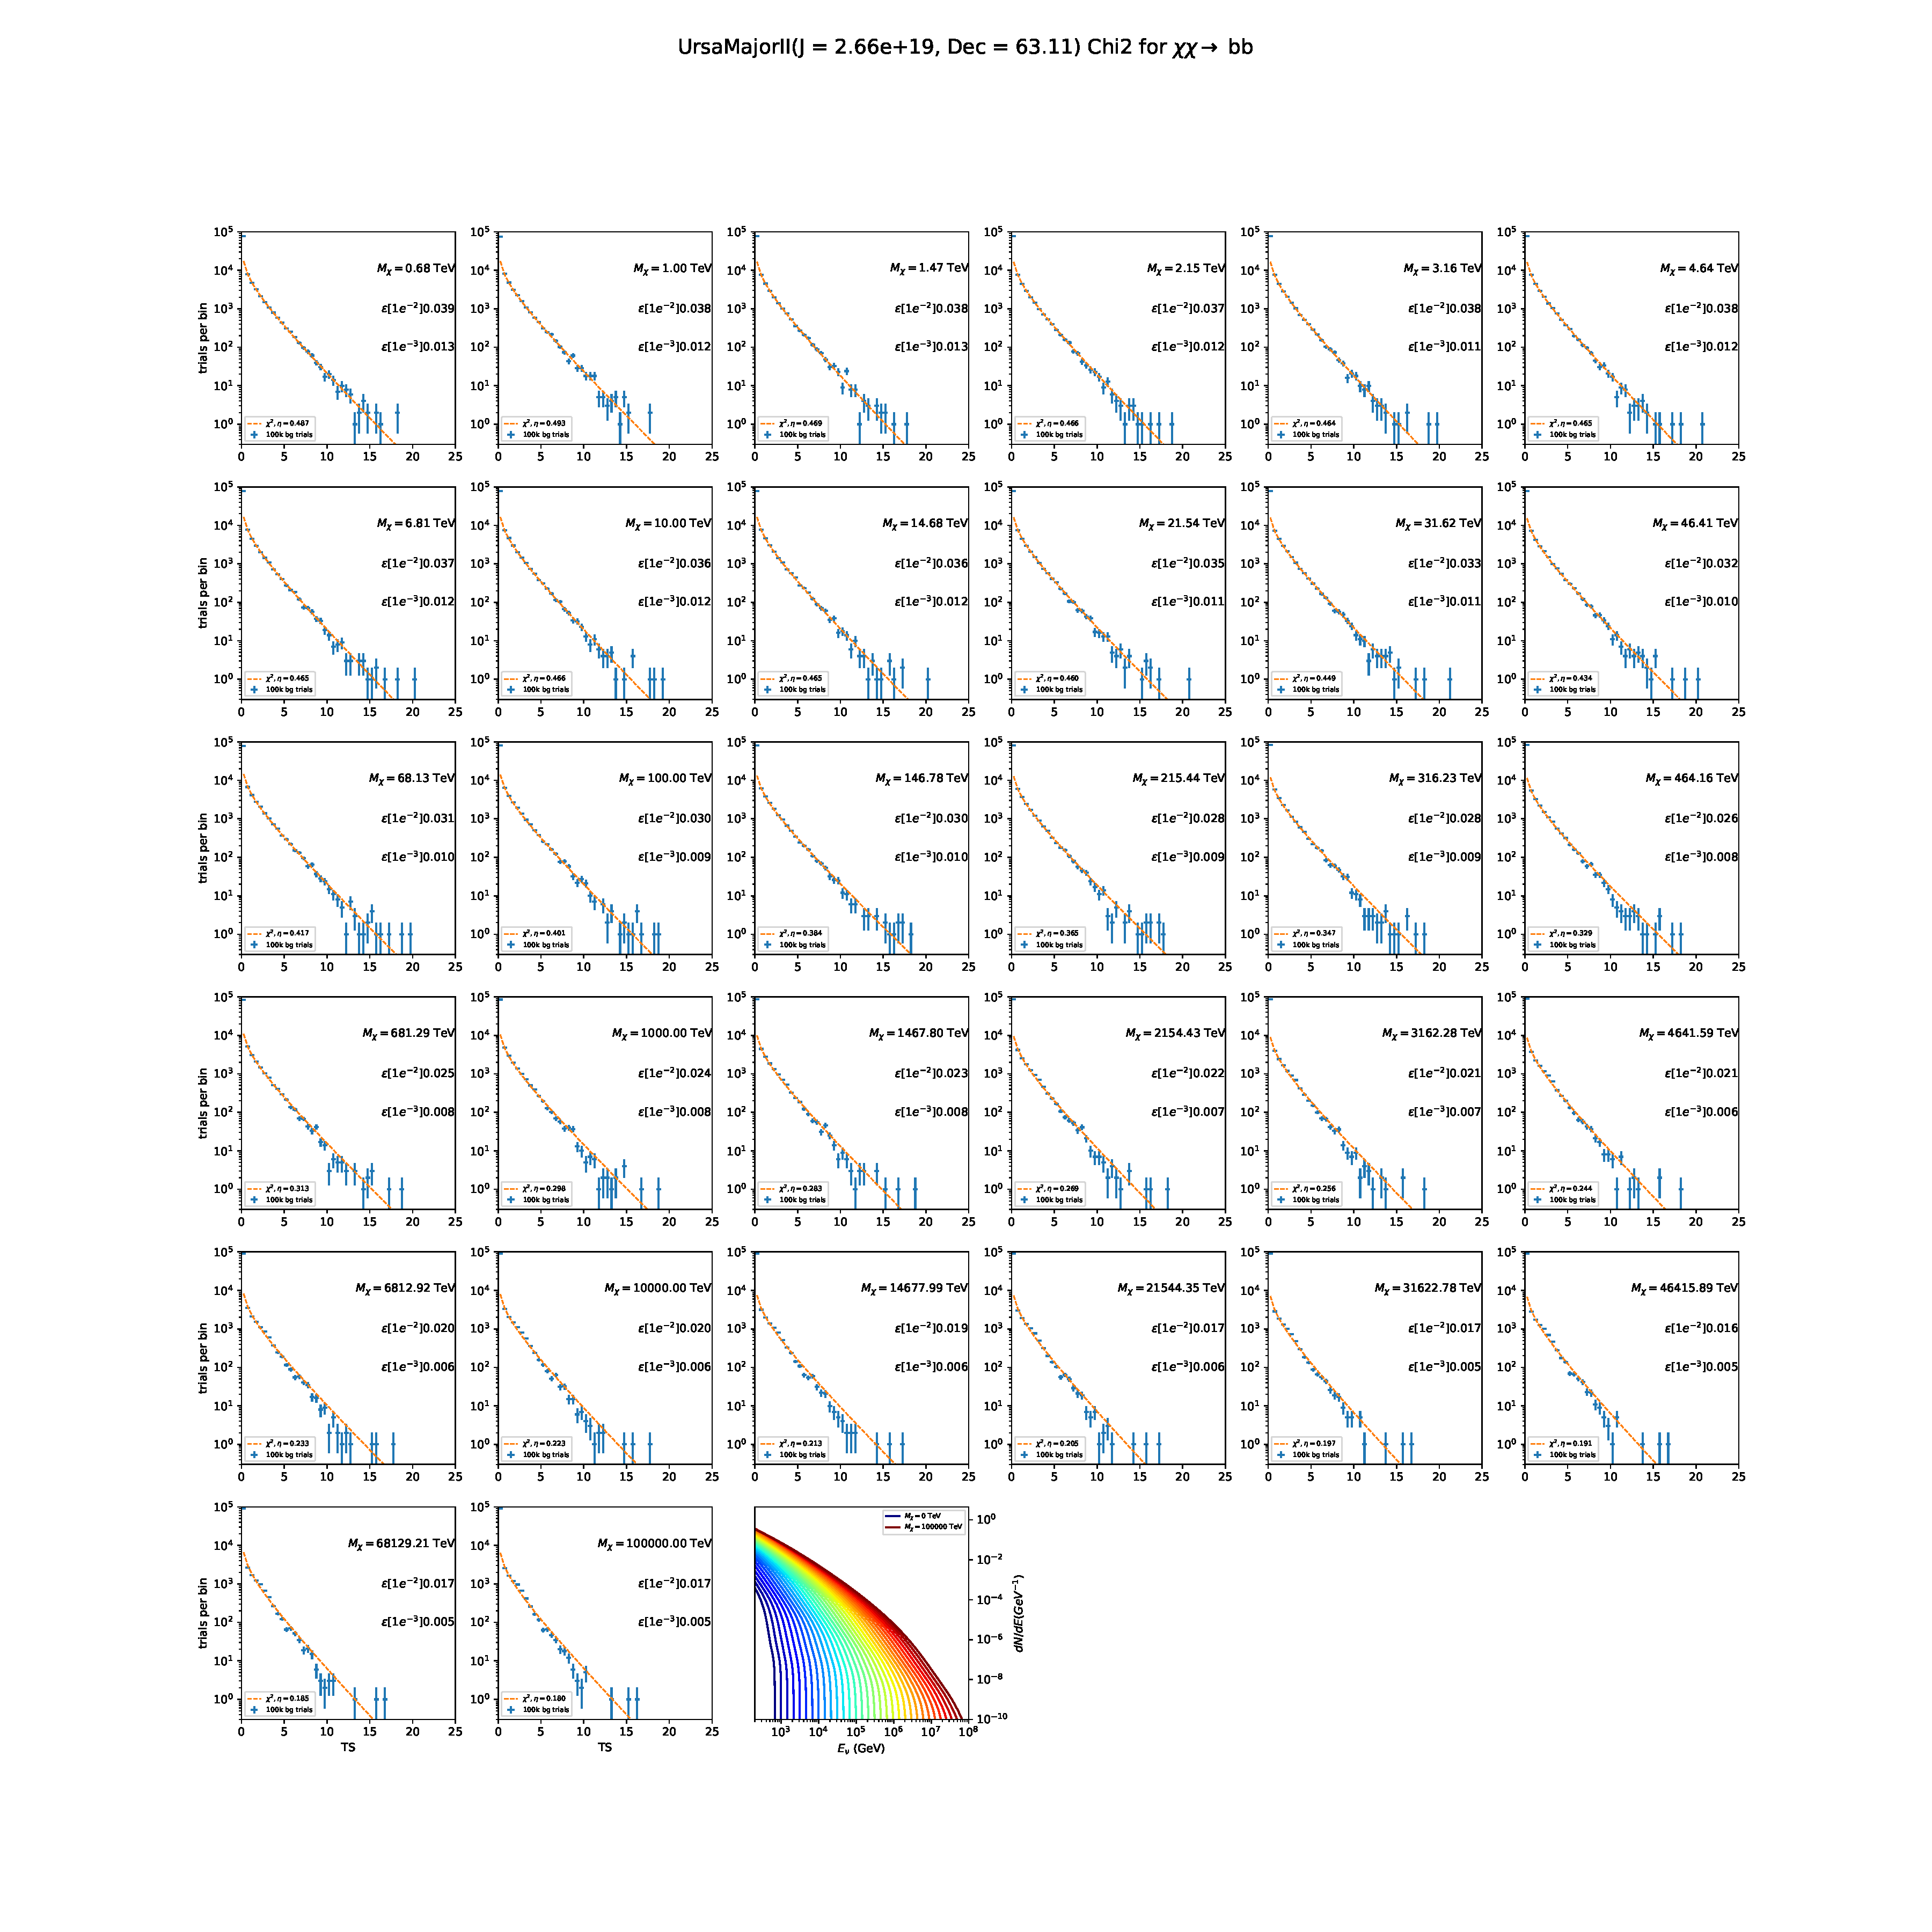
\includegraphics[clip, trim=5.7cm 5.2cm 5.7cm 6.7cm, scale=0.326]{figures/ic_DM/dm_plots/UrsaMajorII_bb_chi2_Masspanel.pdf}
    }\caption{\todo{update text because there is no title.} Each subplot, except the final, is the TS distribution for a specific DM mass listed in the subplot. The final subplot plots the all DM spectral models used as input for the TS distribution calculations with bluer lines indicating lower DM mass and redder indicating higher DM mass.}
    \label{fig:icDM_UMa2bb_TS}
\end{figure}

\begin{figure}[t]
    \centering{
        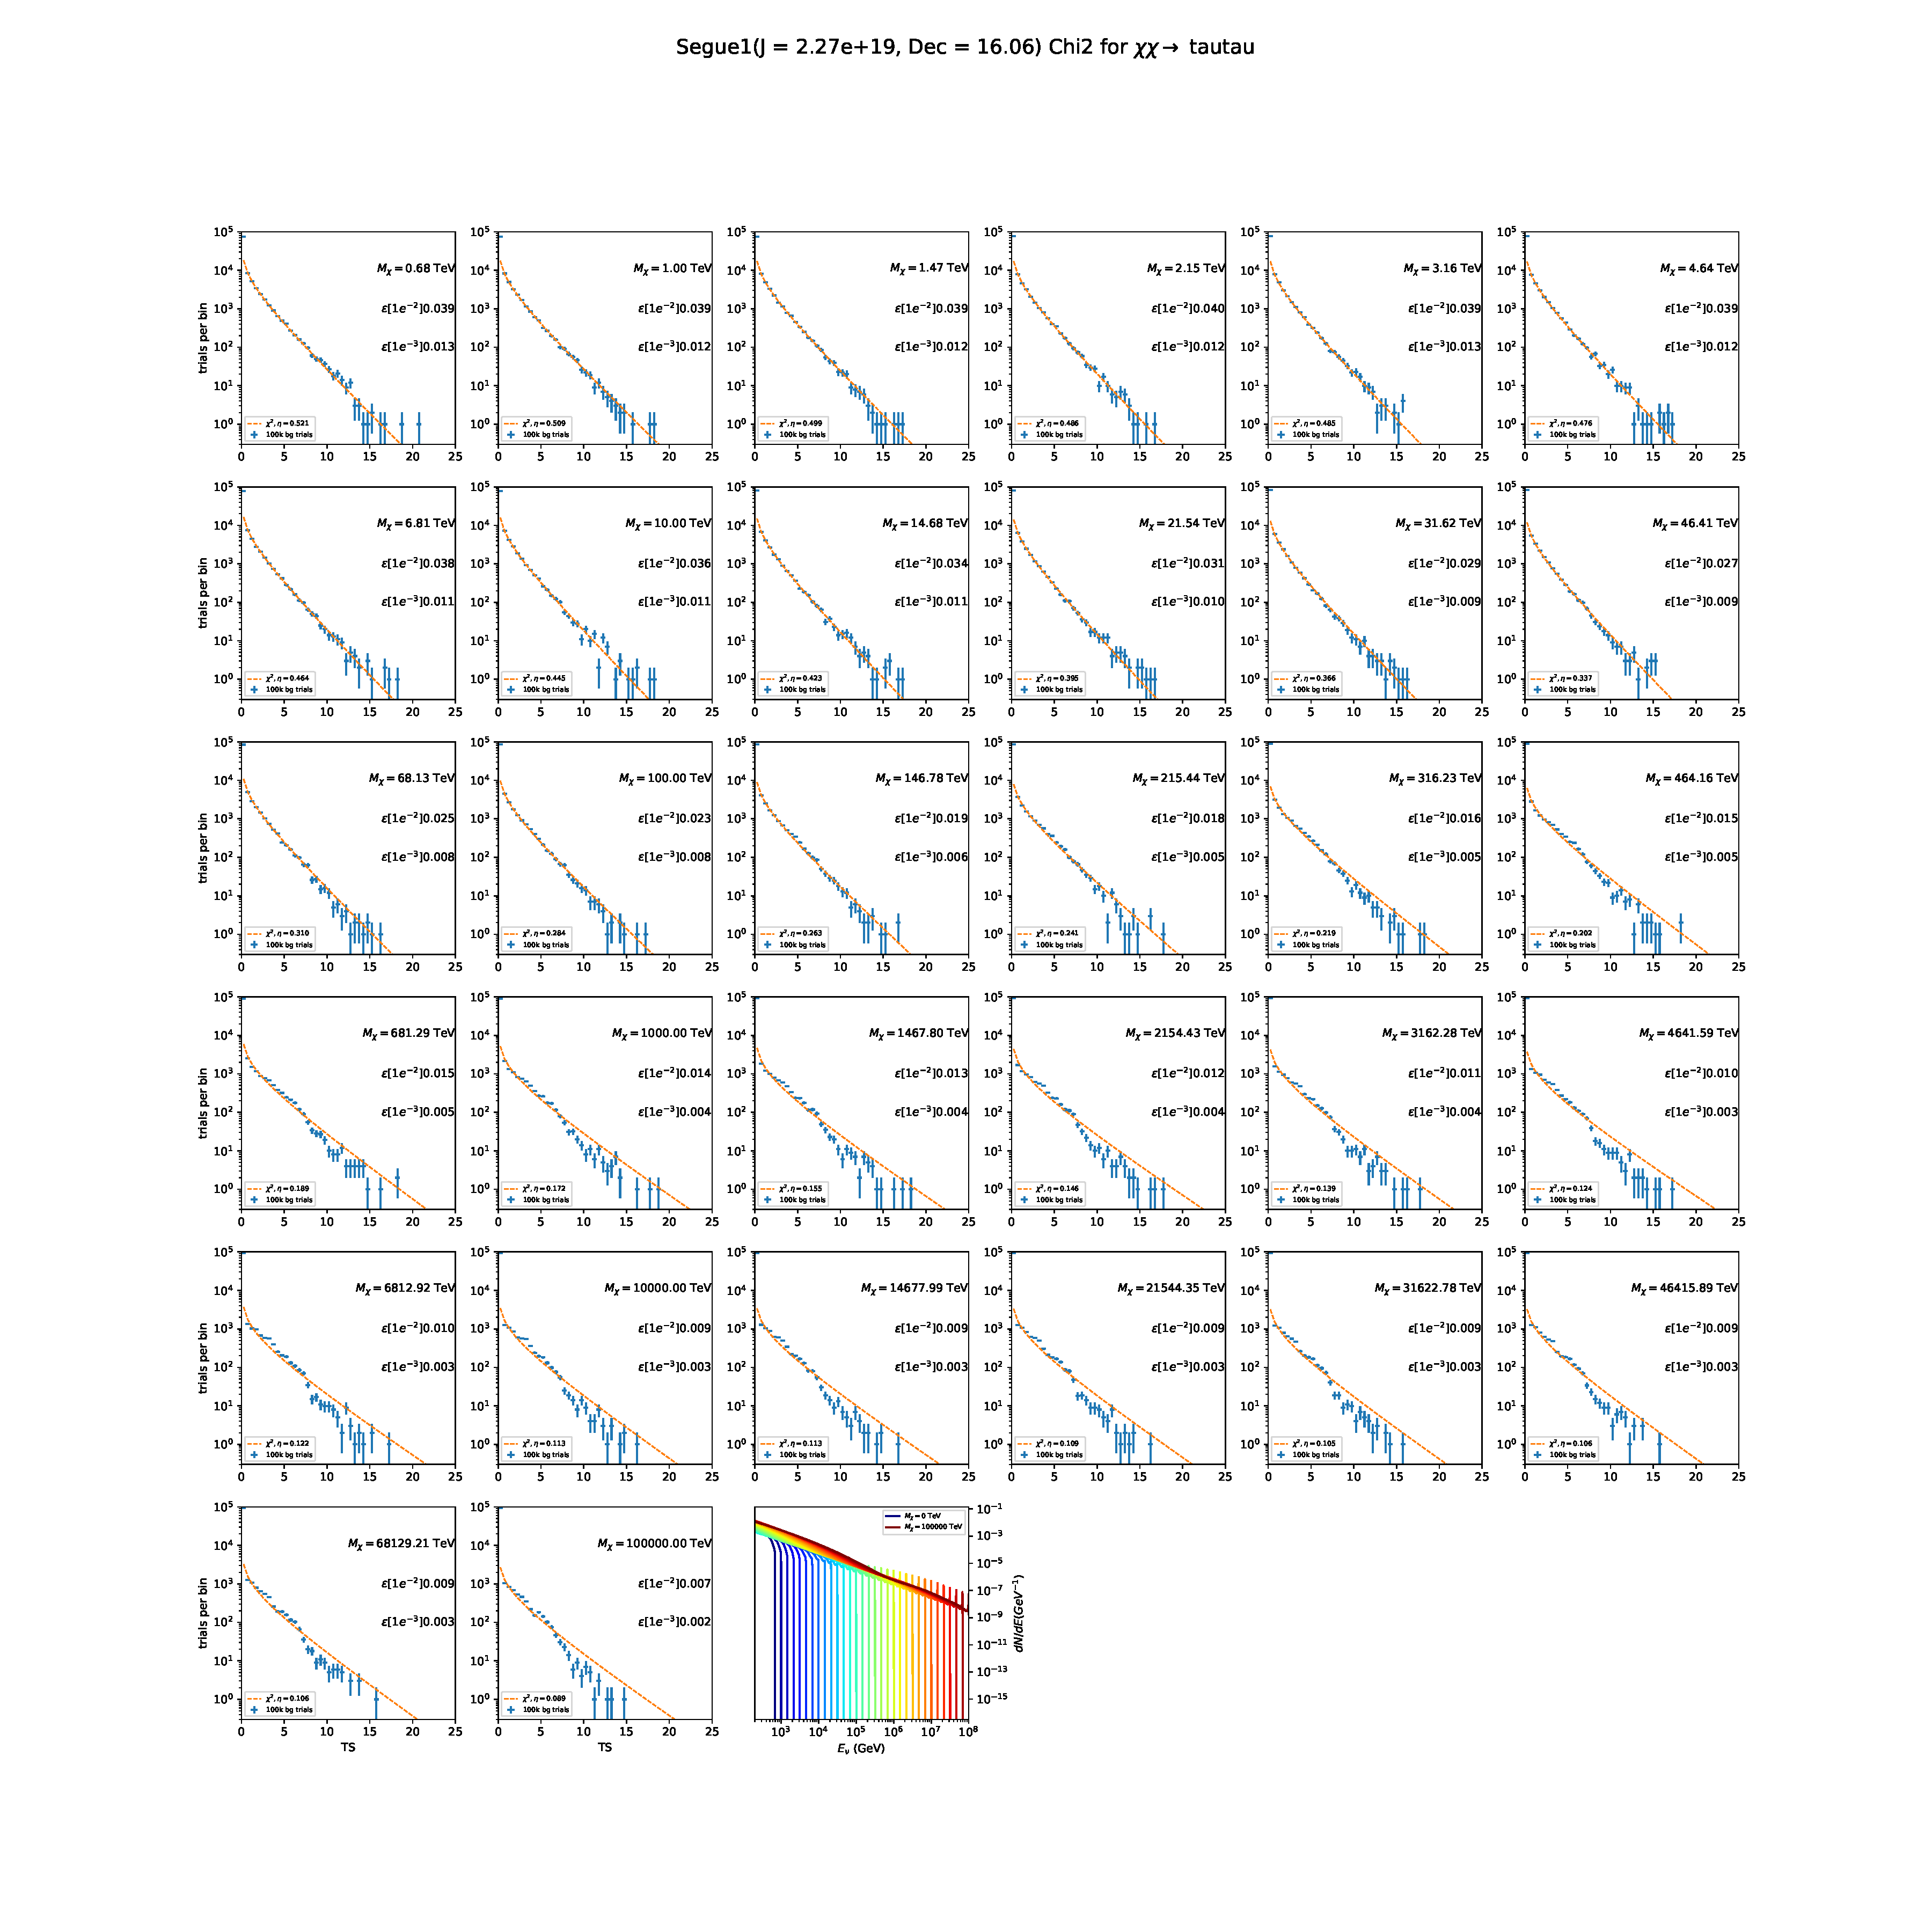
\includegraphics[clip, trim=5.7cm 5.2cm 5.7cm 6.7cm, scale=0.326]{figures/ic_DM/dm_plots/Segue1_tautau_chi2_Masspanel.pdf}
    }\caption{\todo{update text because there is no title.} Each subplot, except the final, is the TS distribution for a specific DM mass listed in the subplot. The final subplot plots the all DM spectral models used as input for the TS distribution calculations with bluer lines indicating lower DM mass and redder indicating higher DM mass.}
    \label{fig:icDM_Seg1tau_TS}
\end{figure}

\begin{figure}[t]
    \centering{
        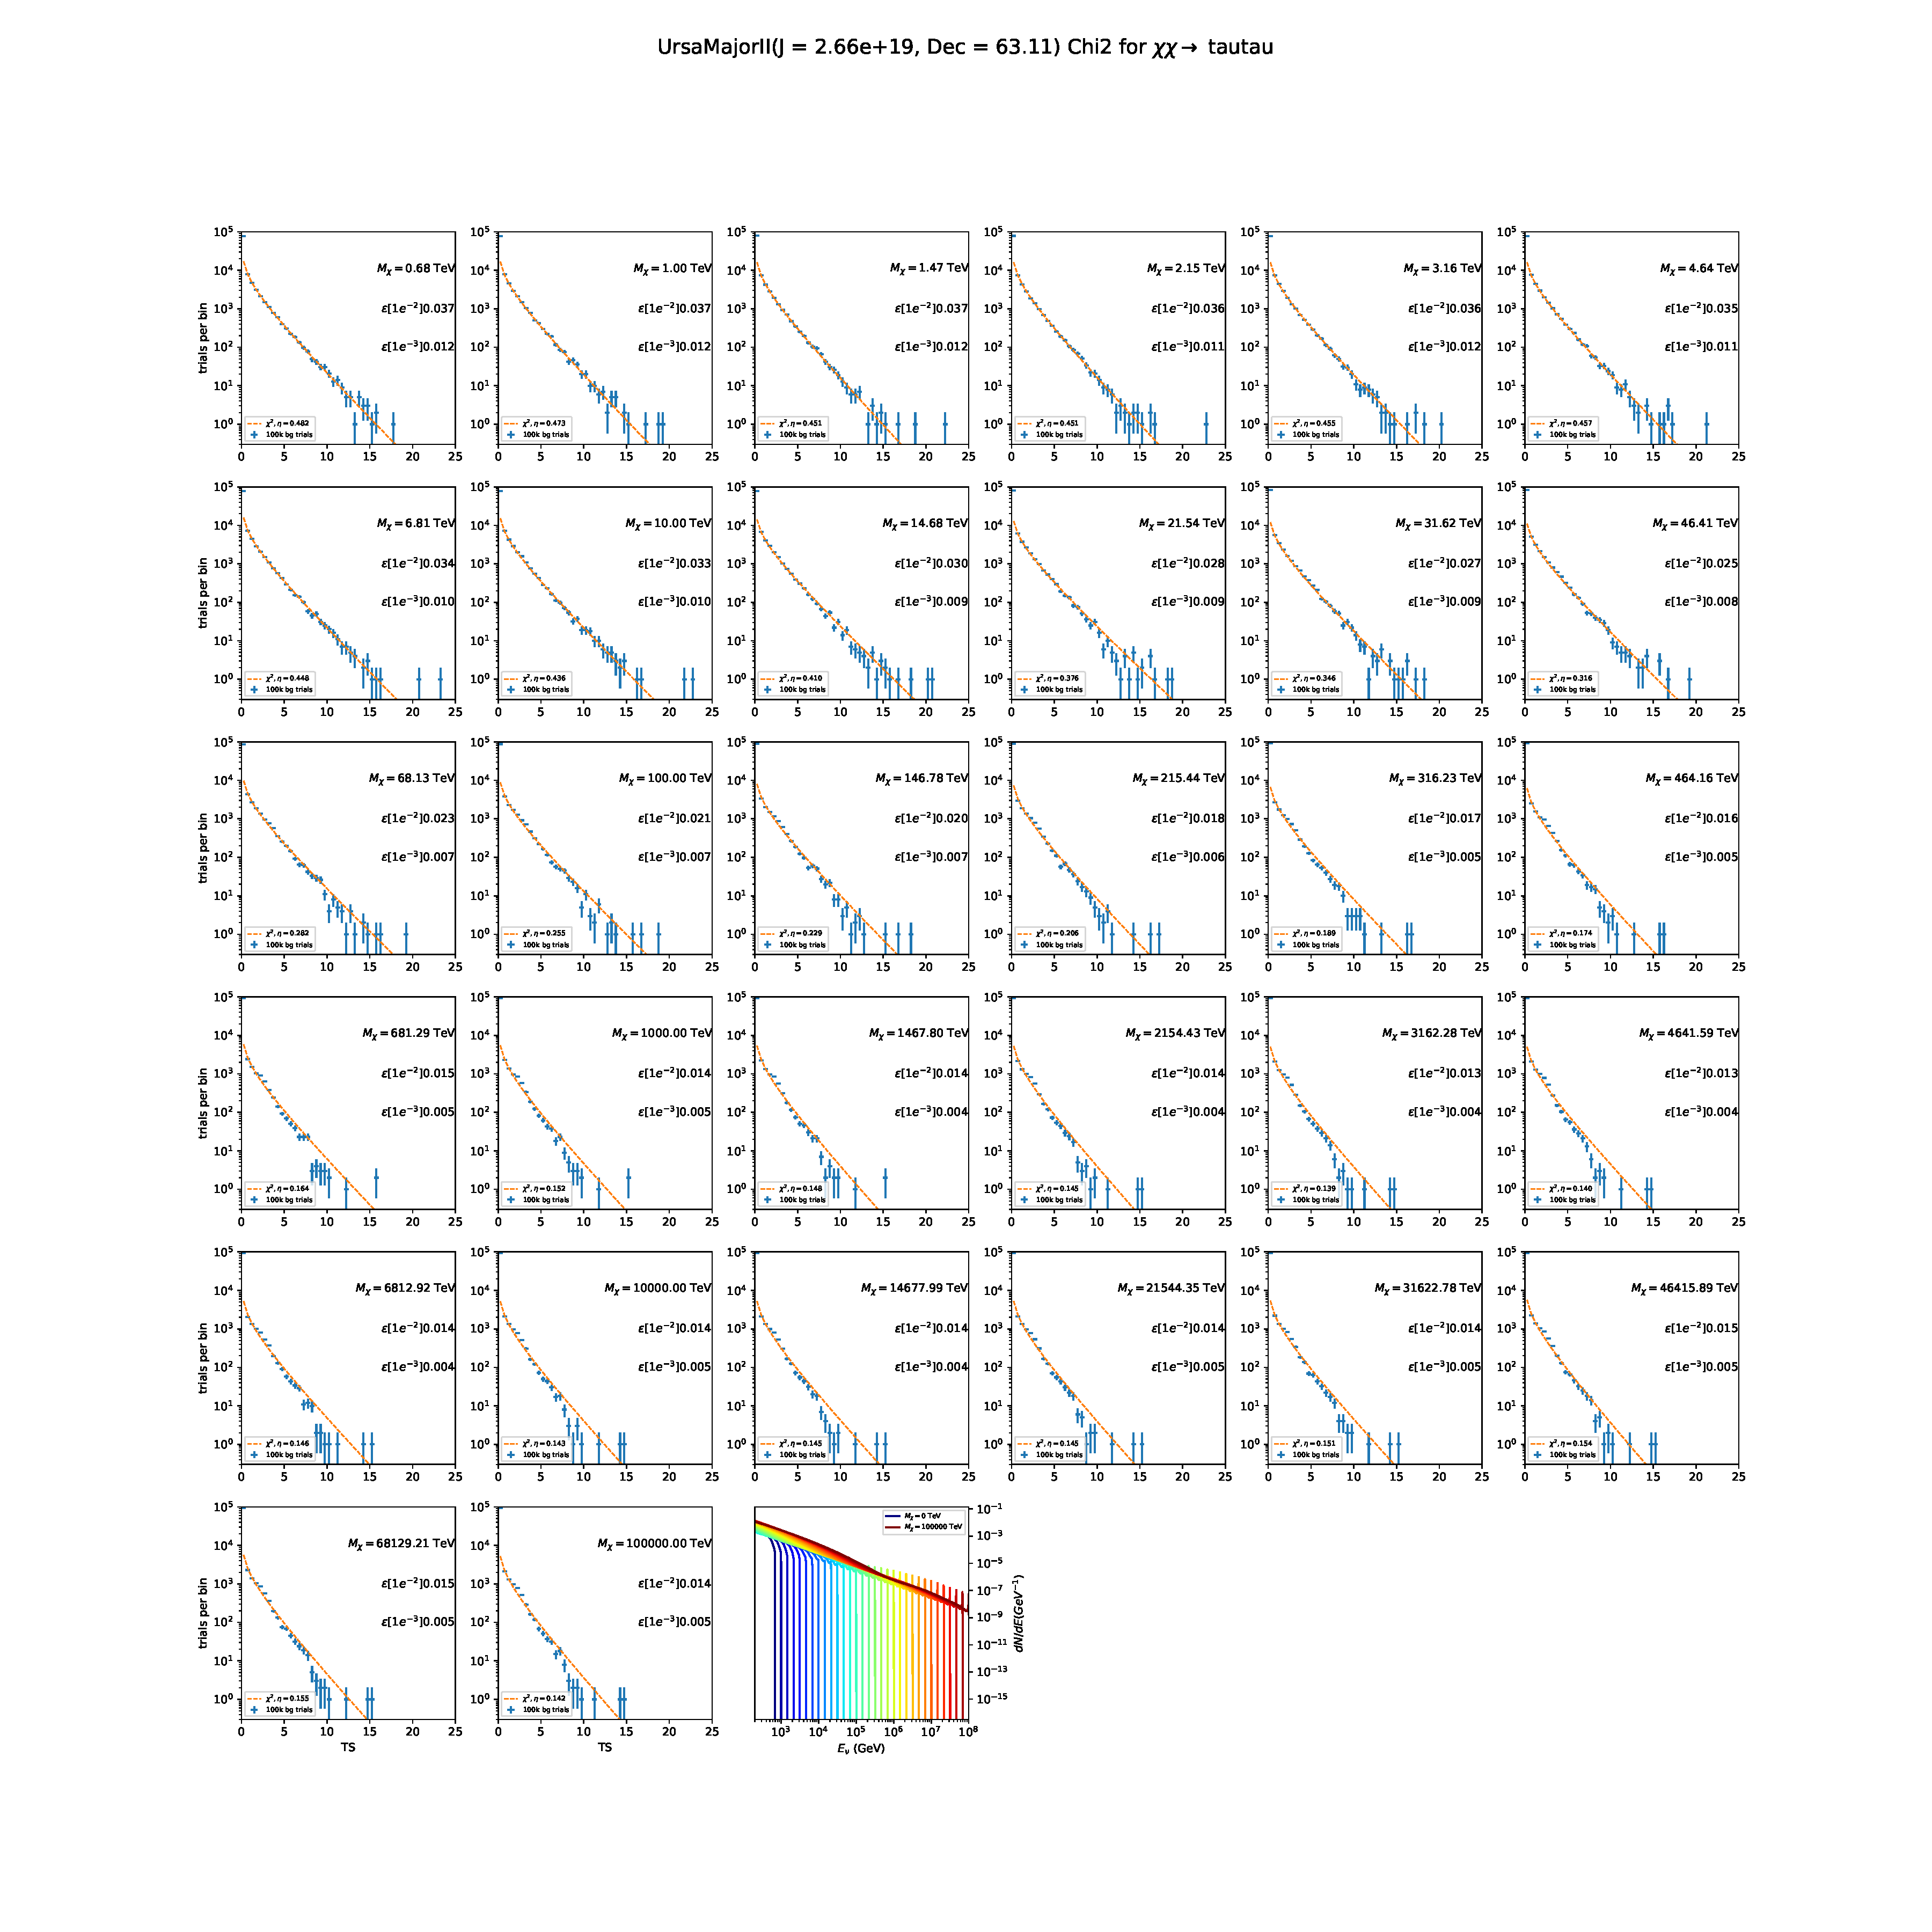
\includegraphics[clip, trim=5.7cm 5.2cm 5.7cm 6.7cm, scale=0.326]{figures/ic_DM/dm_plots/UrsaMajorII_tautau_chi2_Masspanel.pdf}
    }\caption{\todo{update text because there is no title.} Each subplot, except the final, is the TS distribution for a specific DM mass listed in the subplot. The final subplot plots the all DM spectral models used as input for the TS distribution calculations with bluer lines indicating lower DM mass and redder indicating higher DM mass.}
    \label{fig:icDM_UMa2tau_TS}
\end{figure}

\begin{figure}[t]
    \centering{
        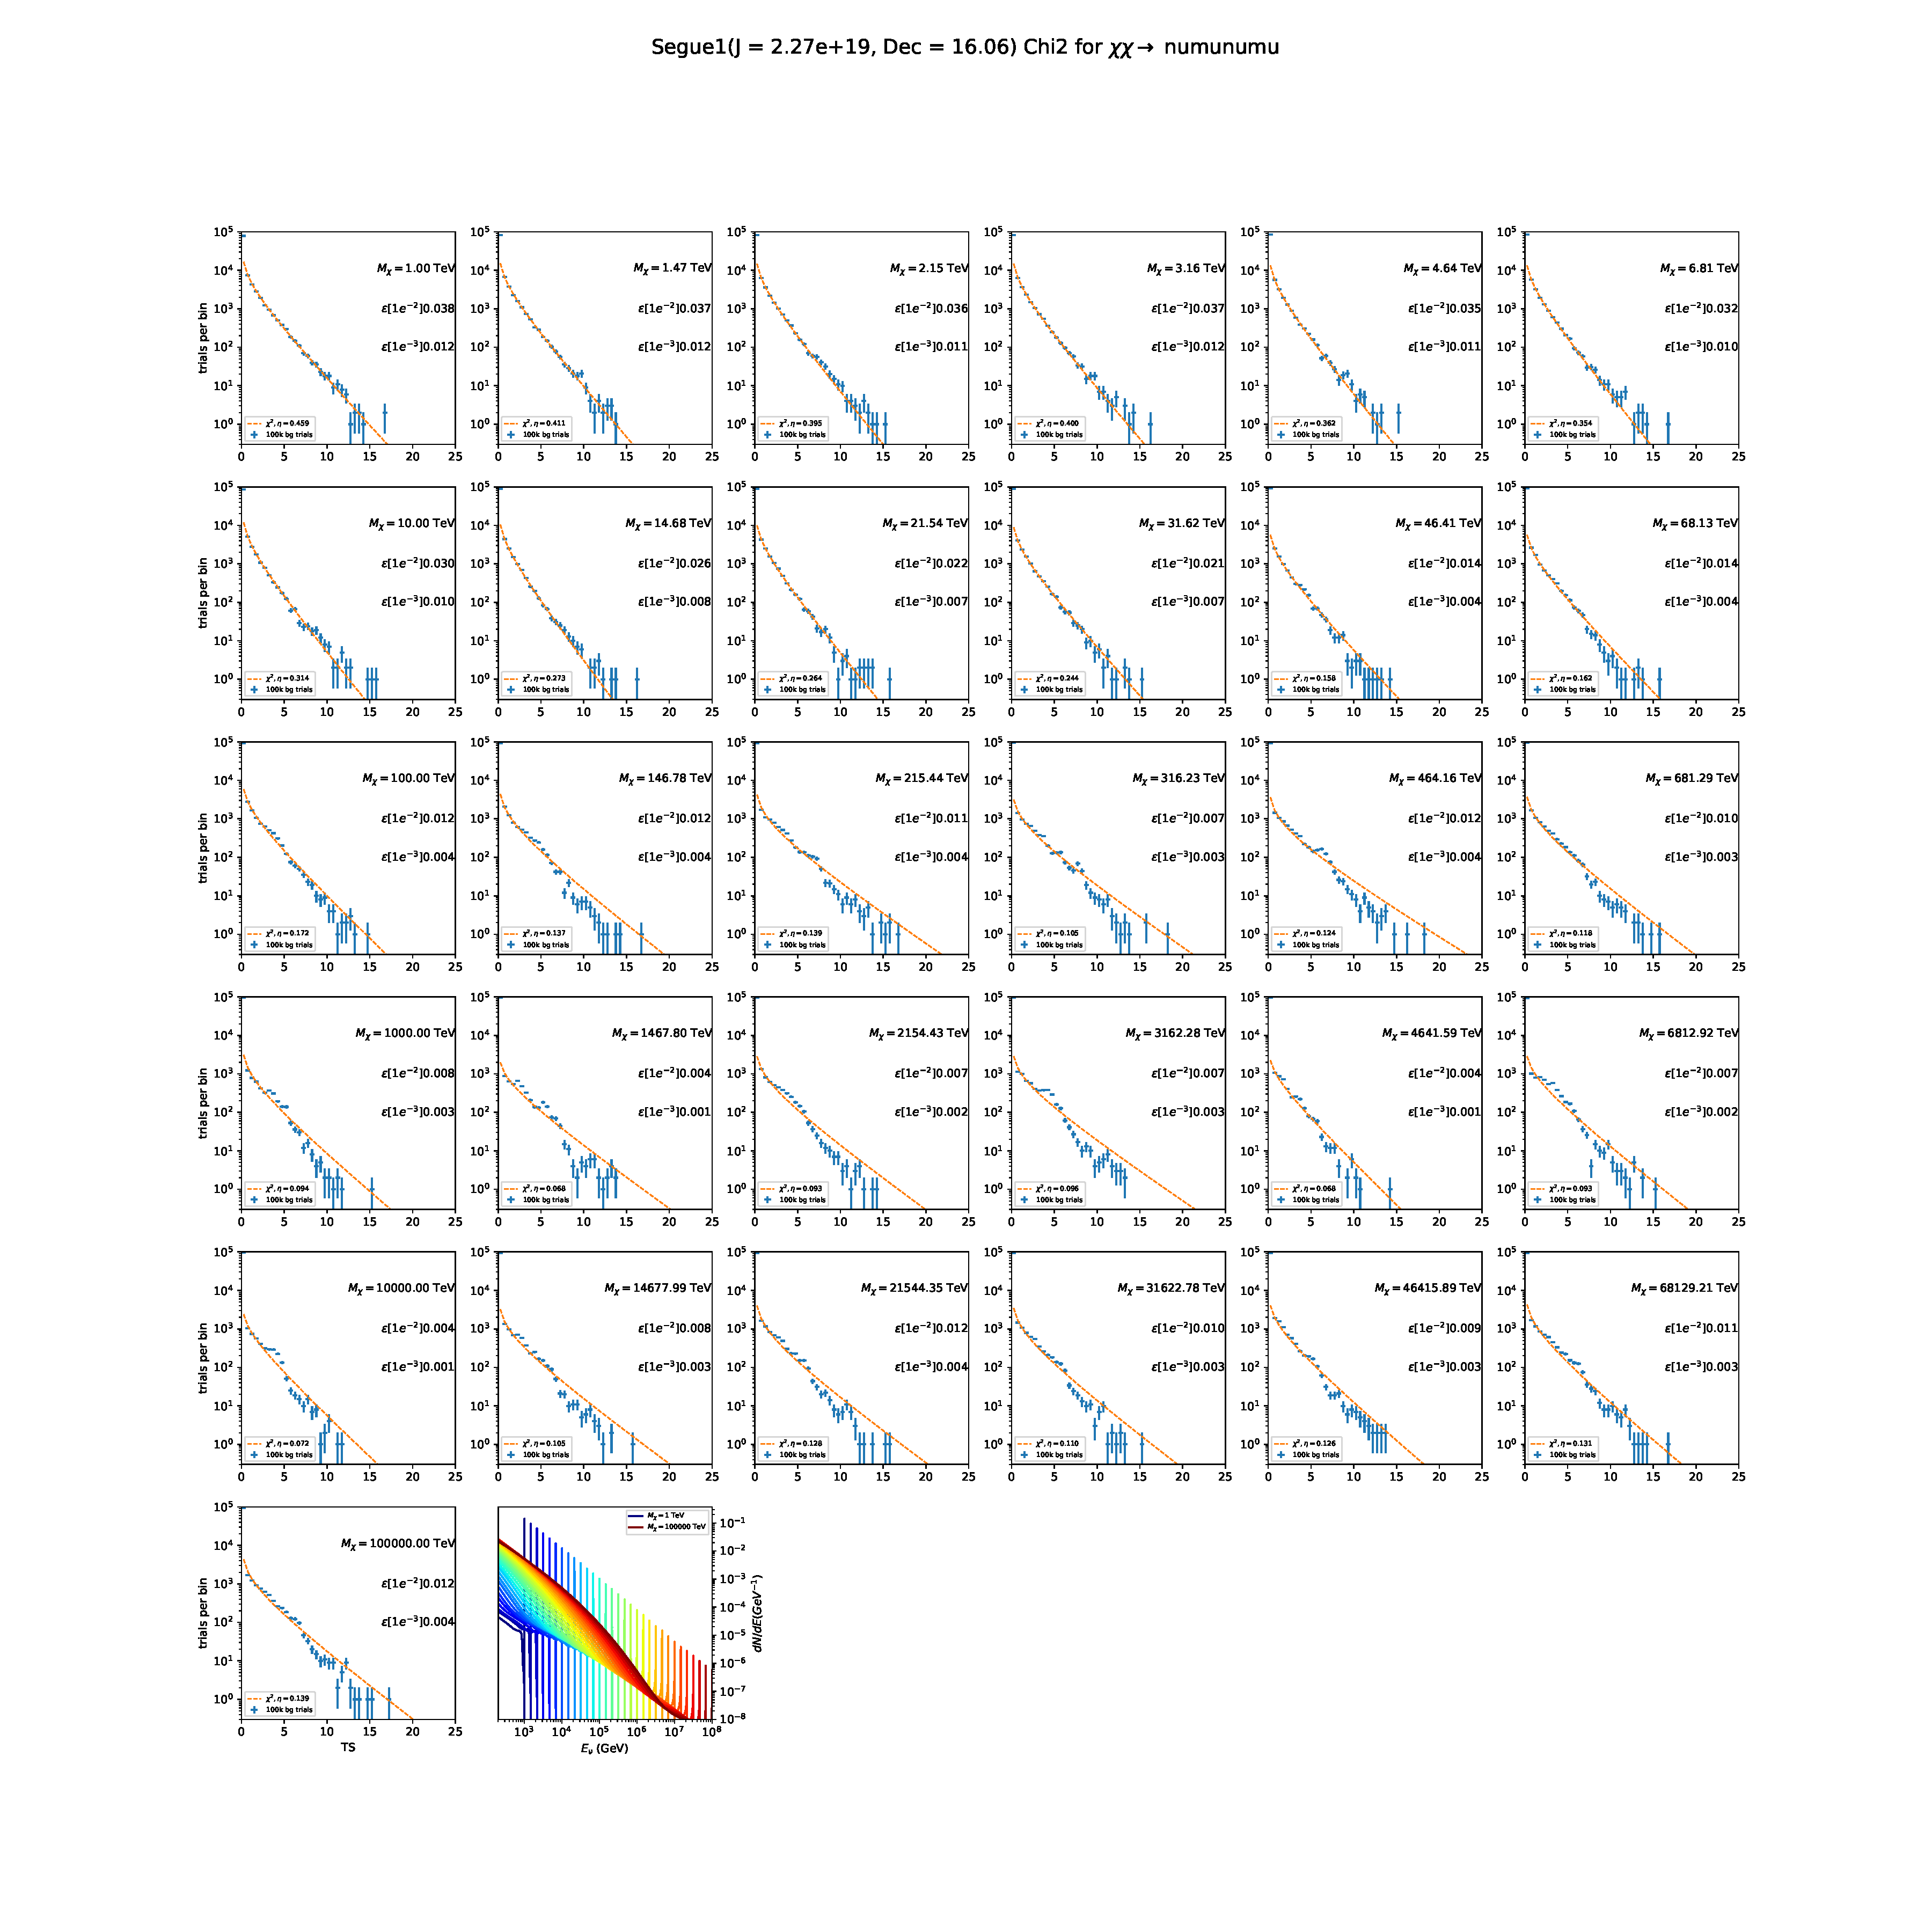
\includegraphics[clip, trim=5.7cm 5.2cm 5.7cm 6.7cm, scale=0.326]{figures/ic_DM/dm_plots/Segue1_numunumu_chi2_Masspanel.pdf}
    }\caption{\todo{update text because there is no title.} Each subplot, except the final, is the TS distribution for a specific DM mass listed in the subplot. The final subplot plots the all DM spectral models used as input for the TS distribution calculations with bluer lines indicating lower DM mass and redder indicating higher DM mass.}
    \label{fig:icDM_Seg1nutau_TS}
\end{figure}

\begin{figure}[t]
    \centering{
        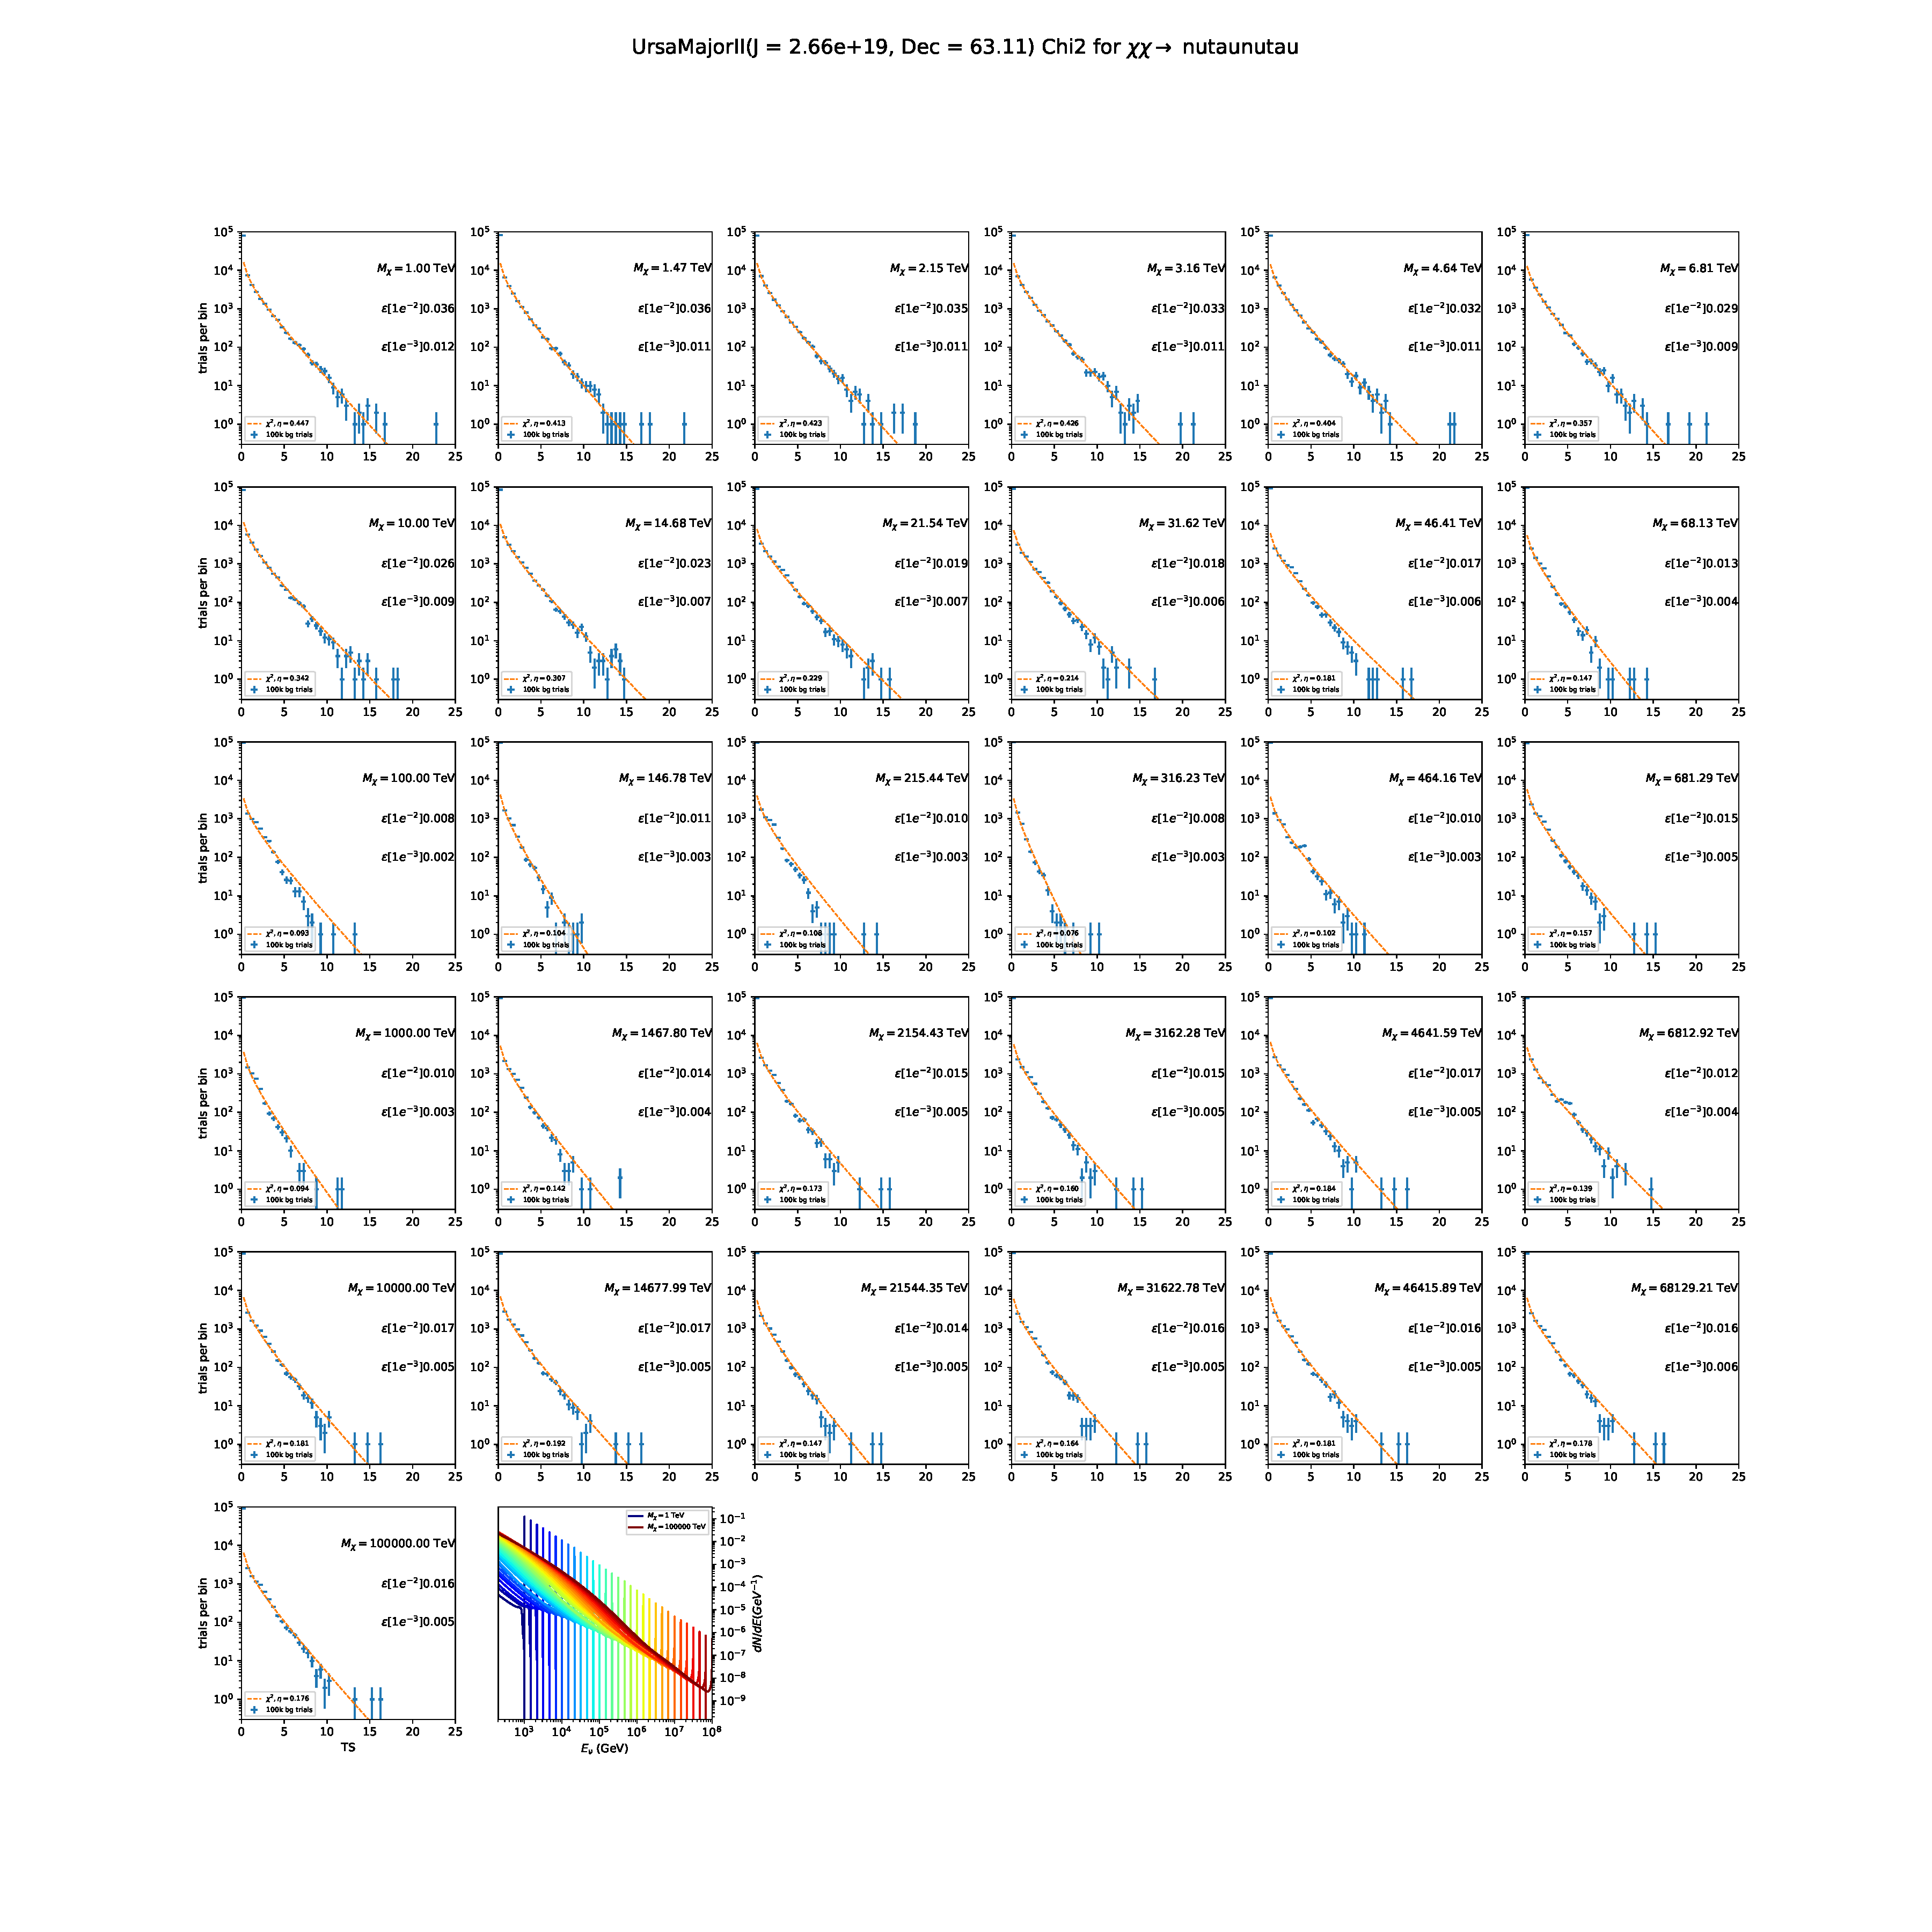
\includegraphics[clip, trim=5.7cm 5.2cm 5.7cm 6.7cm, scale=0.326]{figures/ic_DM/dm_plots/UrsaMajorII_nutaunutau_chi2_Masspanel.pdf}
    }\caption{\todo{update text because there is no title.} Each subplot, except the final, is the TS distribution for a specific DM mass listed in the subplot. The final subplot plots the all DM spectral models used as input for the TS distribution calculations with bluer lines indicating lower DM mass and redder indicating higher DM mass.}
    \label{fig:icDM_UMa2nutau_TS}
\end{figure}
%
% </center>
%
% ==== stacked TS ====
%
% The presentation of these plots are identical to the previous 'per Source' section. I use csky source software to calculate the TS distributions.
% Bugs were found when implementing, however were rectified. Warning to future users performing a stacked analysis with custom spectra.
% In using the above, I am making the implicit assumption that the primary/only cause to a difference in neutrino counts from the sources is accounted for through the J-factors.
% The J-factors are therefor used as weights for the stacking where an individual source's weight is defined as:
%
% <center>
% <big>$ w_i = \frac{J_i}{\sum^{N_\mathrm{sources}}_{k=1}J_k} $</big>
% </center>
%
% where $ w_i $ is the ith source, $ J_{i/k} $ is the i/k-th source's J-factor.
%
% Below is the TS distribution for each SM annihilation channel with stacking of 15 sources.
%
% [[Media: stacked_bb_chi2_Masspanel.pdf | $ b\overline{b} $ 1/7/2024]]
%
% [[Media: stacked_ww_chi2_Masspanel.pdf | $W^+W^- $ 1/7/2024]]
%
% [[Media: stacked_zz_chi2_Masspanel.pdf | $Z^0 Z^0 $ 1/7/2024]]
%
% [[Media: stacked_tt_chi2_Masspanel.pdf | $ t\overline{t} $ 1/7/2024]]
%
% [[Media: stacked_nuenue_chi2_Masspanel.pdf | $ \nu_e\overline{\nu_e} $ 1/7/2024]]
%
% [[Media: stacked_numunumu_chi2_Masspanel.pdf | $ \nu_\mu\overline{\nu_\mu} $ 1/7/2024]]
%
% [[Media: stacked_nutaunutau_chi2_Masspanel.pdf | $ \nu_\tau\overline{\nu_\tau} $ 1/7/2024]]
%
% Each subplot, except the final, is the TS distribution for a specific DM mass listed in the subplot. The final subplot plots the all DM spectral models used as input for the TS distribution calculations with bluer lines indicating lower DM mass and redder indicating higher DM mass.
% Below is an image of bb. The full resolution pdfs were provided in links above.
%
% <center>
% [[Image: stacked_bb_chi2_Masspanel.jpeg| 800px ]]
%
% </center>
%
% === Signal Recovery ===
%
% This did have a lot of plots before but the spectra have change substantially since then. They converge well but since the computational is expensive here, I'm holding off on rerunning until the spectra are finalized.
%
% === Sensitivities ===
%
% In IceCube, we usually define the 90% confidence level (CL), as the minimum number of signal events (n_s) required to have a Type I error rate smaller than 0.5 and Type II error rate of 0.1.
% Csky performs the sweep to find n_s that satisfies the previous condition, and from n_s I use the following equation
%
% <center>
% $
% n_{s} = T_{live} \int_{0}^{\Delta\Omega}d\Omega \int_{E_{min}}^{E_{max}} dE_{\nu} A_{eff}(\hat{n}, E_{\nu}) \frac{d \Phi_{\nu}}{d\Omega d E_{\nu}} (\hat{n}, E_{\nu}),
% $
% </center>
%
% to extract the sensitivity on the dark matter annihilation cross-section.
% $ T_{live} $ is the detector livetime, $ A_{eff} $ is the effective area of the detector, and $ E_{min} $, $ E_{max} $ are the minimum, maximum energies of the expected neutrinos, respectively.
%
% Sensitivities are calculated for each source individually as if they were the only source and as a stack.
% Example plots of these plots are shown below and organized by the single source/stacked studies.
% Finally, I generated a plot with all hypotheses which is presented at the very end.
%
% ==== per Source ====
%
% ==== Stacked ====
%